\documentclass[a4paper,12pt,oneside]{report}
\usepackage{a4wide}
\usepackage{ucs}
\usepackage[utf8x]{inputenc}
\usepackage{xcolor}
\usepackage[czech,english]{babel}
\usepackage[pdftex, final]{graphicx}
\usepackage{alltt}
\usepackage{paralist}
\usepackage{mdwlist}
\usepackage{subfig}
\usepackage[final]{pdfpages}
\usepackage[final,pdftex, colorlinks=false]{hyperref}

%\usepackage{pdfpages}
\usepackage{perpage} %the perpage package
%\MakePerPage{footnote} %the perpage package command

\usepackage{amsmath}
%\usepackage{hyperref}
\usepackage{acronym}

\usepackage[font={small}]{caption}
\usepackage{multirow}
\usepackage{fancyvrb}
\usepackage{subfig}
\usepackage{titlesec}
\usepackage{listings}

\usepackage{footmisc}

\makeatletter
\def\verbatim@font{\linespread{1}\normalfont\ttfamily}
\makeatother



%%%%%%%%%% fancy %%%%%%%%%%%
\usepackage{fancyhdr}

\fancyhead[L]{ČVUT v Praze}

\setlength{\headheight}{16pt}

% \usepackage{stdpage}

%cislovani kapitol
\renewcommand*\thesection{\arabic{section}}
\renewcommand{\chaptername}{}
\renewcommand{\thechapter}{}
%\titleformat{\chapter}{\normalfont\huge}{}{20pt}{\huge\textbf}

\renewcommand{\partname}{}
\renewcommand{\chaptername}{}



%%%%%%%%%%%% rozmery %%%%%%%%%%%%%%%%%%
\usepackage[%
%top=40mm,
%bottom=35mm,
%left=40mm,
%right=30mm
top=40mm,
bottom=35mm,
left=35mm,
right=25mm
]{geometry}


\renewcommand\baselinestretch{1.3}
\parskip=0.8ex plus 0.4ex minus 0.1 ex

%%%%%%%%%%%%%% Listings %%%%%%%%%%%%%%%%%
%%\usepackage[final]{listings}

\definecolor{lightGrey}{RGB}{250,250,250}
\definecolor{darkGrey}{RGB}{100,100,100}
\lstdefinelanguage{psmap}
{morekeywords={scale, mapinfo, maploc, where, end, font, fontsize, color,
border, raster, width, paper,
vpoints, vareas, vlines, symbol, size, rgbcolumn, sizecolumn, cwidth,
rotatecolumn, },
morekeywords=[2]{y, n, none},
morecomment=[l]{\#},
}



\lstdefinestyle{script}{
    language=bash,
    basicstyle={\ttfamily\footnotesize},
    keywordstyle={\bfseries},
    commentstyle={\itshape},
    frame=lines,
    backgroundcolor=\color{lightGrey}
}
\lstnewenvironment{psmap}[1][]
{\lstset{style=psmap,
   #1}}
   {}
\renewcommand{\lstlistingname}{Ukázka}

\lstdefinestyle{mybash}{
   language=bash,
   basicstyle={\ttfamily},
   keywordstyle=[1]{\bfseries},
   keywordstyle=[2]{\color{black}},
   commentstyle={\itshape},
   frame=lines,
   showstringspaces=false,
   backgroundcolor=\color{lightGrey},
}

\lstdefinestyle{python}{
   language=python,
   basicstyle={\ttfamily},
   keywordstyle=[1]{\bfseries},
   keywordstyle=[2]{\color{black}},
   commentstyle={\itshape},
   frame=lines,
   showstringspaces=false,
   backgroundcolor=\color{lightGrey},
}










%%%%%%%%%%%%%%%%%%%%%%%%%%%%%%%%%

\newcommand{\klicslova}[2]{\noindent\textbf{#1: }#2}
\newcommand{\modul}[1]{\emph{#1}}
%\newcommand{\instr}[1]{\lstinline[style=psmapInline]|#1|}
\author{Matěj Krejčí}
% \pagecolor{darkGrey}
\newcommand{\necislovana}[1]{%
\phantomsection
\addcontentsline{toc}{section}{#1}
\section*{#1}
\markboth{\uppercase{#1}}{}
}


%%%%%%%%%%%%%%%%%%%%%%%%%%%%%%
\begin{document}
\pagestyle{empty}
%nastaveni velikosti footnote
\renewcommand\footnotelayout{\footnotesize}
\pagenumbering{gobble}
\begin{center}
%napisy
\newcommand{\napisCVUT}{České vysoké učení technické v Praze}
\newcommand{\napisFS}{Fakulta stavební}
\newcommand{\napisObor}{Obor geoinformatika}
\newcommand{\napisKatedra}{Katedra geomatiky}
\newcommand{\napisVedouci}{Ing. Martin Landa Ph.D.}
\newcommand{\napisAutor}{Matěj Krejčí}
\newcommand{\napisDatum}{Praha 2014}
\newcommand{\napisNazevI}{Analýza a vizualizace srážkových dat }
\newcommand{\napisNazevII}{z mikrovlnných telekomunikačních spojů pomocí GIS}
\newcommand{\napisNazevAjI}{Analysis and vizualization of rainfall data from}
\newcommand{\napisNazevAjII}{microwave links using GIS}
\newcommand{\napisBakalarka}{Bakalářská práce}
\newcommand{\napisPraha}{Praha 2014}
%
% prikazy
%\newcommand{\velka}[1]{\uppercase{#1}}
\newcommand{\velka}[1]{\textsc{#1}}
%
% 
\newif\ifpatitul
\patitultrue

\ifpatitul
{\Large\velka{\napisCVUT}}\\
\velka{\Large\napisFS}\\
\vfill
{\LARGE\velka{\napisBakalarka}}
\vfill
{\large\napisPraha\hfill\napisAutor}
\newpage
\fi%patitul


{\Large\velka{\napisCVUT}}\\
{\Large\velka{\napisFS}}\\
{\Large\velka{\napisObor}}
\vfill

\includegraphics[width=3cm]{logo_cvut_cb} %~
\vfill
{\Large\velka{\napisBakalarka}}\\
{\Large\velka{\napisNazevI\\
\napisNazevII}}\\
{\large\velka{\napisNazevAjI\\
\napisNazevAjII}}
\vfill
{\large%
Vedoucí práce: \napisVedouci\\
\napisKatedra\\
\bigskip
\napisDatum\hfill\napisAutor}
\end{center}

\newpage
\definecolor{navodotisk}{RGB}{10,10,10}
\newcommand{\vlozZadani}{%
\Huge\textcolor{navodotisk}{\textsf{\textbf{ZDE VLOŽIT ORIGINÁLNÍ ZADÁNÍ}}}%
}
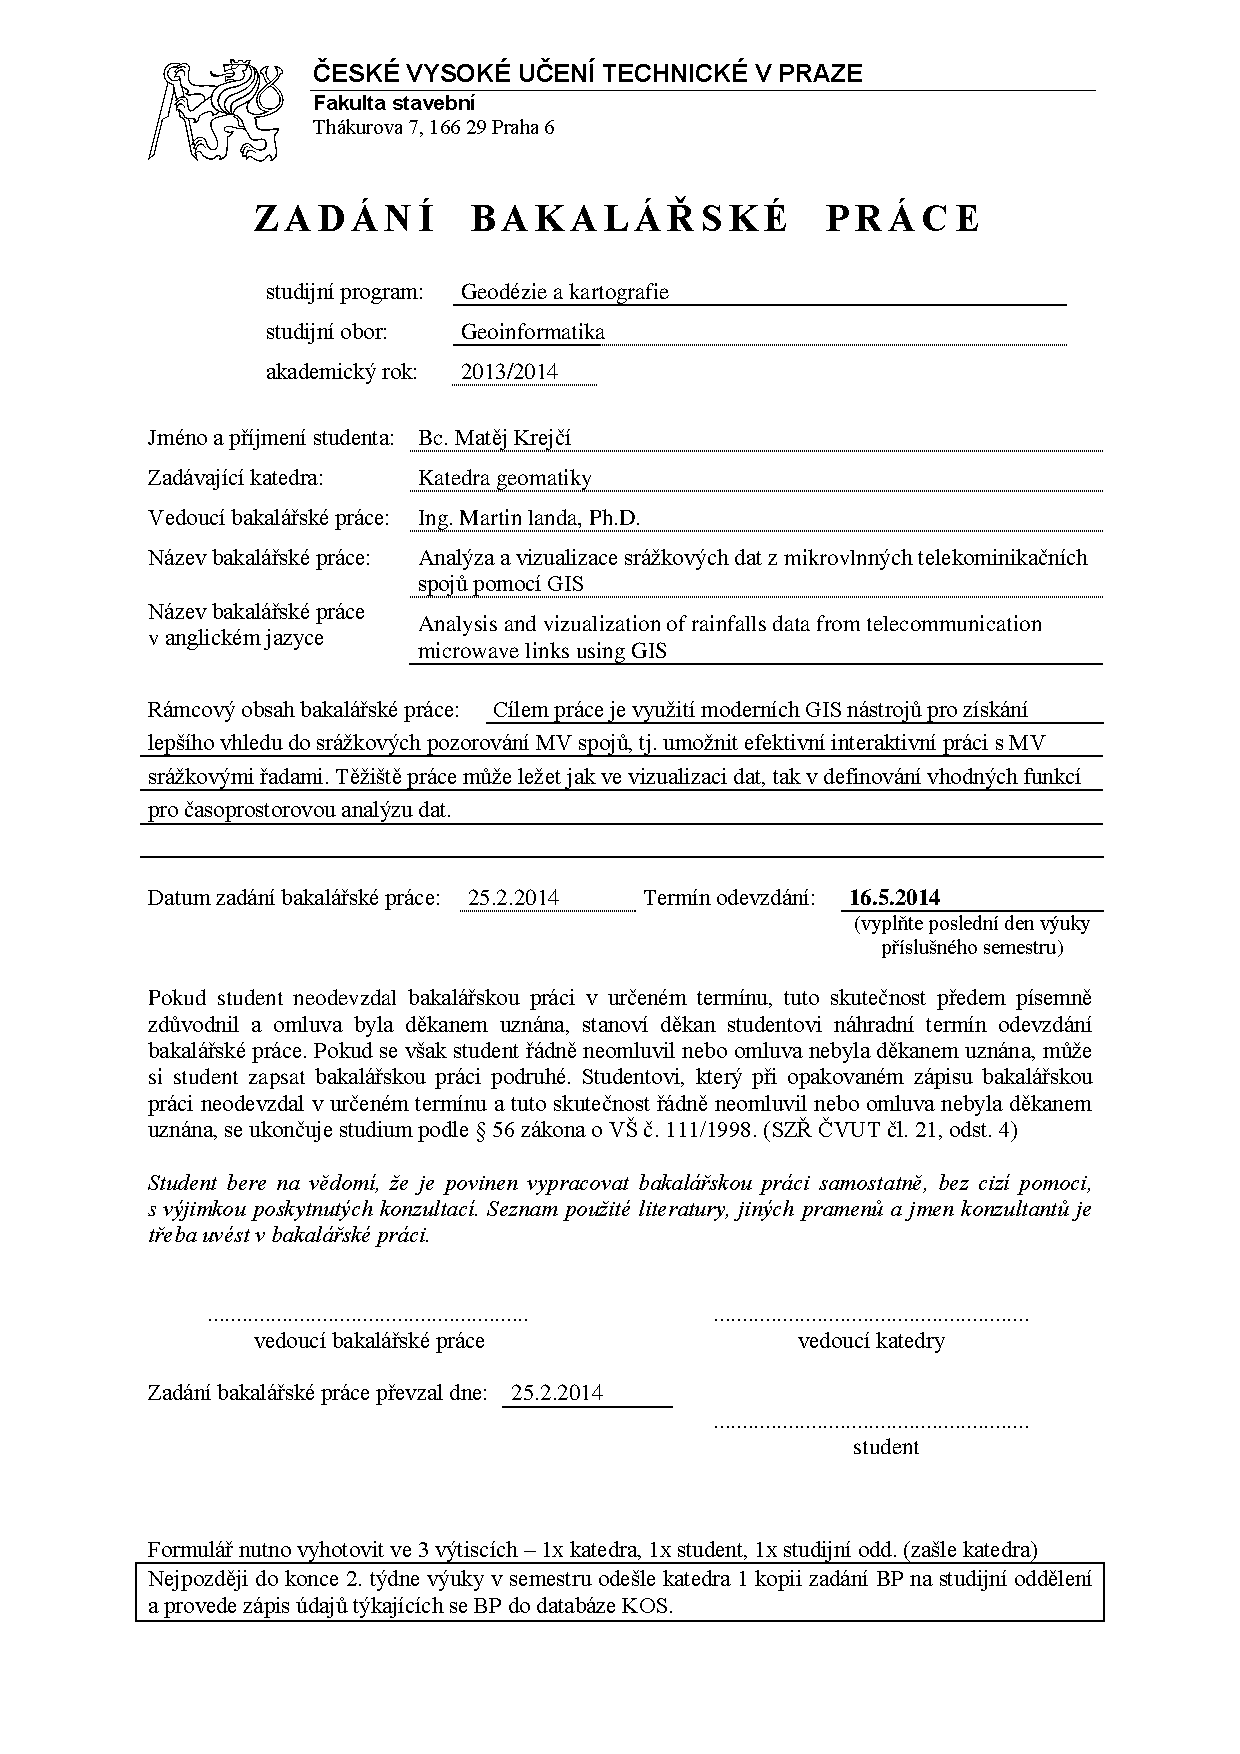
\includepdf[picturecommand={\put(100,200){\vlozZadani}}]{../formulare/zadanibp}
 % resi si zalomeni sam


\begin{abstract}
Cílem této bakalářské práce je modelování dešťových srážek z dat mikrovlnných spojů telekomunikačních operátorů. Data ke zpracování jsou uložena pomocí relační databáze PostgreSQL.
K vývoji modulu byl použit systém \textit{GRASS Python Scripting Library}. Modul implementuje rekonstrukce dešťových srážek na základě uživatelské konfigurace. Další funkcionalitou je dávkové zpracování grafického výstupu srážek. Hlavní přínos modulu spočívá v procesu primárního zpracování dat pro následné analýzy v hydrologii a meteorologii s využitím nástroje GIS.
\bigskip

\klicslova{Klíčová slova}{GIS, GRASS GIS, Python, PostgreSQL, dešťové srážky, časoprostorová analýza, interpolace}

\end{abstract}

\selectlanguage{english}
\begin{abstract}
TODO 
\bigskip

\klicslova{Keywords}{GIS, GRASS GIS, Python, PostgreSQL, precipitation, temporal analysis,interpolation}

\end{abstract}
\selectlanguage{czech}


\newpage
\newcommand{\odsaditodzhora}{\hskip1pt\vfill}

\odsaditodzhora
\noindent Prohlášení
%%% MK: predelano po revizi
Prohlašuji, že bakalářskou práci na téma „Analýza a vizualizace srážkových dat z mikrovlnných telekomunikačních spojů pomocí GIS“ jsem vypracoval samostatně. Veškerá použitá literatura je uvedena v seznamu zdrojů.

\begin{flushleft}
\begin{tabular}{cp{0.3\textwidth}c}
V Praze dne .................
& 
&
..................................
\\
&&
(podpis autora)
\end{tabular}

\end{flushleft}
\newpage

\odsaditodzhora
\noindent Poděkování

Tady bude podekovani

\newpage

\newpage

\tableofcontents


\newpage
\necislovana{Úvod}

\pagestyle{fancy}

\pagenumbering{arabic}
\setcounter{page}{1}
\subsection*{Předmluva}
Enviromentální procesy jsou součástí planety Země od jejího vzniku. Obvykle jsou tyto procesy komplexního charakteru a pro jejich pochopení je nutné souhrnných  studií. S vývojem informačních technologií jsou dostupné ke studiu problematik stále sofistikovanější metody, které umožňují komplexnější přístup a pochopení jevů v širším kontextu. Mezi sofistikované metody se bezesporu řadí fyzikální či numerické modely, které umožňují výpočty které by bez výpočetních kapacit nebyly možné. Informační technologie v současné době dosahují velkého rozmachu a výpočetní výkonnost se mezi desetiletími mění ve stovkách až tisících procent. Tento fakt umožňuje využívat metod, které by před dekádou nebyly reálné.

Modely, které simulují přírodní procesy jsou pro jejich komplexnost charakteristické velikými objemy dat, které je nutné spravovat a analyzovat. V posledních desetiletích velmi usnadňují práci nastroje geografických informačních systémů (GIS), které se jsou všeobecně dostupné a umožňují vysokou variabilitu ve správě a analýze dat. Jednotlivé nástroje GIS z pravidla nebývají úzce zaměřené na komplexní problematiky, ale jejich návaznost a možné propojení s vlastními aplikacemi ulehčuje vytvoření komplexních nástrojů.

\subsection*{Motivace}
Modelování dešťových srážek je jednou z disciplín z oboru enviromentálního modelování. Když se poohlédneme do první poloviny 19. století, tak právě meteorologie byla jednou z prvních disciplín, která definovala pojem enviromentální modelování, tak jak ho chápeme nyní. Rekonstrukce srážek na zemském povrchu se s vývojem klimatu stává v poslední době důležitým úkolem. Oproti rozvoji fyzikálně numerických modelů nebyl technologický pokrok ve sběru srážkových dat v posledních desetiletích takřka zaznamenán. Pracovníky meteorologických a hydrologických ústavů ve vývoji brzdí nedostatečně přesná a neaktuální srážková data, která jsou jedním z hlavních vstupů pro další modely. Studie z posledních let poukazují na možnost využití mikrovlnných (MV) spojů vysílačů telekomunikačních operátorů ke sběru srážkových dat. Jedním z velkých  potenciálů sběru přesných srážkových dat v reálném čase je  zlepšit výsledky  městských odtokových modelů. Pro efektivitu těchto modelů je sběr dat v dostatečném rozlišení a v reálném čase nutností.

\subsection*{Cíl}
Hlavním cílem této práce je vývoj nástroje pro zpracování hrubých dat z MV vysílačů v prostředí GIS, čímž se zpřístupní nespočet dalších analýz které napomůžou výzkumu těchto nových metod. Sekundárně je práce zaměřena na využití výstupů vlastního GIS nástroje k grafické interpretaci plošných srážek. Přímo na to navazující je definování vhodných časoprostorových funkcí nástroje GIS. Téma práce bylo založeno na požadavcích zpracovatele projektu, který se zabývá problematikou odhadu srážek z MV spojů v rámci projektu "TeleMAS"\footnote{GA ČR 14-22978S Predikce srážkového odtoku v urbanizovaných povodích na základě deštěm generovaného útlumu signálu mikrovlnných spojů telekomunikační sítě} v souvislosti s modelováním srážko-odtokových procesů v městských povodích. Tento projekt je řešen v úzké vědecké spolupráci s ETH-Eawag a odborné spolupráci se společnostmi T-Mobile a Veolia ČR a nyní nově s Ericsson Research (Sweden).

Práce je systematicky rozdělena na část teoretickou a praktickou. V teoretické části je kladen důraz na představení základních pojmů a principů, důležitých pro část praktickou. Praktická část je obsahuje  představení funkcionality vlastních GIS modulů a využití jejich funkcionalit společně se stávájícími nástroji GIS.

 



\newpage
\chapter*{Teoretická část}\stepcounter{chapter}\addcontentsline{toc}{chapter}{Teoretická část}
Tato kapitola je úvodem k praktické části práce a je zaměřena na nástroje využité k implementaci Python modulu do GRASS GIS. Jsou zde popsány základní principy a charakteristiky jednotlivých nástrojů, kde je kladen především důraz na návaznost k praktické části práce.



\paragraph*{Geografické informační systémy} současné doby, poměrně efektivně umožňují správu a analýzu srážkových dat. Jejich funkce jsou vhodné jak pro správu dat, tak pro její analýzu a vizualizaci. Jednotlivec metody měření srážek jsou specifické svojí datovou charakteristikou z prostorového a časového pohledu. 

Metody měření srážek jsou svoji charakteristikou dat rozdílné. Srážkoměry produkují bodová data v rázných časových intervalech, výstupem z radaru jsou snímky představující intenzitu srážek a satelitní družice produkují nespočet specifických druhů dat. Společné mají to, že je třeba jejich výstupy někde spravovat a analyzovat. GIS nástroje umožňují tyto požadavky splňovat poměrně dostatečně a částečně eliminují potřebu vývoje specifických systémů, který by měli obecně stejný základ.

Charakteristikou moderních GIS je především veliká disponibilita dílčích funkcí, které jednotlivě nemají velkou sílu, ale ve spojení umožňují rozsáhle analýzy. V případě že ve sledu funkcí některé nedostačují k řešení daných problematik, bývá obecně u většiny vyspělých systémů možnost vývoje vlastních GIS aplikací s využitím stávajících funkcí. Díky tomu je v dnešní době celkem dostupné vyvíjet specifické funkce pro GIS, bez nutnosti vývoje rozsáhlých základů programů GIS.



\section{Úvod do měření dešťových srážek}
Úvod této kapitol má za cíl přiblížit současné metody měření dešťových srážek. Liší se především v přesnosti, časové variabilitě a vhodností výstupu pro další využití. Úvod do problematiky měření srážek poukazuje na klady a zápory metody odhadu srážek pomocí MV.


\paragraph*{Dešťové srážky}jsou definovány jako produkt vodní páry v kapalném nebo pevném stavu, které padají z oblohy či kondenzují přímo na zemském povrchu. Srážky mohou mít formu sněhových vloček - pevné skupenství, nebo formu dešťových kapek - kapalné skupenství. Množství srážek bývá udáváno v milimetrech kapalné vody spadlé na zemský povrch za časový interval.\cite{wmo} 

\subsection{Současné nástroje a metody }
\label{subsec:11}

\subsubsection{Srážkoměry}
Srážkoměr je přístroj používaný v meteorologii a hydrologii k měření srážkových úhrnů. Dle funkčnosti se srážkoměry dělí na dešťové a na srážkoměry, které měří i srážky pevného skupenství. Tyto srážky se přeměňují na ekvivalent vody a až poté se měří. Důležité je podotknout, že produktem srážkoměrů jsou bodová srážkoměrná data.

\subsubsection{Meteorologický radar}
Radarová měření díky plošnému pokrytí a dobrému prostorovému i časovému rozlišení dat jsou vhodná pro synoptickou a leteckou meteorologii. Poskytují přehled v reálném čase o pohybu a struktuře srážkových systémů, umožňují velmi krátkodobou předpověď v řádech minut až hodin a z ní plynoucí varování před nebezpečnými meteorologickými jevy.\cite{radar_chmu}

\paragraph*{Srážková data} se měří obvykle v intervalu 5-15 minut. Horizontální rozlišení dat bývá 2×2 km, vertikální 1 km. Toto prostorové rozlišení je nutné, aby bylo možné zachytit jednotlivá srážková jádra přeháněk. Radarové odrazy jsou interpretovány plošně a jsou zobrazovány v barevné stupnici intenzit srážek.

\paragraph*{Rozsah} meteorologického radaru bývá okolo 250 km. Hodnoty naměřené radarem mohou být použity pro odhad okamžitých intenzit srážek do vzdálenosti přibližně 150 km od radaru.\cite{kohout}

\subsubsection{Dálkový průzkum země}
Je důležité zmínit možnost získávání informací o srážkách pomocí \acs{DPZ}. Tento obor z hlediska meteorologie zaujímá zcela jiný náhled na měření srážek oproti předchozím metodám. \acs{DPZ} v meteorologii umožňuje globální pohled na meteorologické jevy. Makro náhled na enviromentální jevy, např. cyklóny, tropické bouře, tornáda či pohyb mraků, je podstatný pro sledování a pochopení globálního vývoje klimatu. Do této kategorie spadá pozorování pomocí družic na oběžných drahách a leteckých prostředků pohybujících se v zemské atmosféře. 


\subsection{Mikrovlnné spoje}
Mikrovlnné (MV) spoje jsou rádiové systémy široce využívané v oblasti telekomunikací (zejména 
mobilními operátory) k bezdrátovému propojení dvou vzdálených stanovišť. MV spoje operují na 
frekvencích, kde dešťové kapky představují hlavní zdroj útlumu signálu. Analýza útlumu signálu 
umožňuje poměrně přesně odhadnout průměrnou srážkovou intenzitu podél spoje. Vzhledem 
k hustotě sítě MV spojů (např. v Praze řádově stovky až tisíce) jde o relevantní zdroj srážkové 
informace, který má velký potenciál zlepšit prostorovou informaci o srážkových intenzitách. Využití 
standardních GIS nástrojů může výrazně zefektivnit jak zpracování dat, tak jejich následnou správu. 
Vhodná vizualizace těchto dat je důležitým předpokladem pro vylepšení stávajících modelů pro 
převod útlumu signálu MV spojů na srážkové intenzity i pro další využití těchto dat.
 
\begin{figure}[h!]
    \centering
    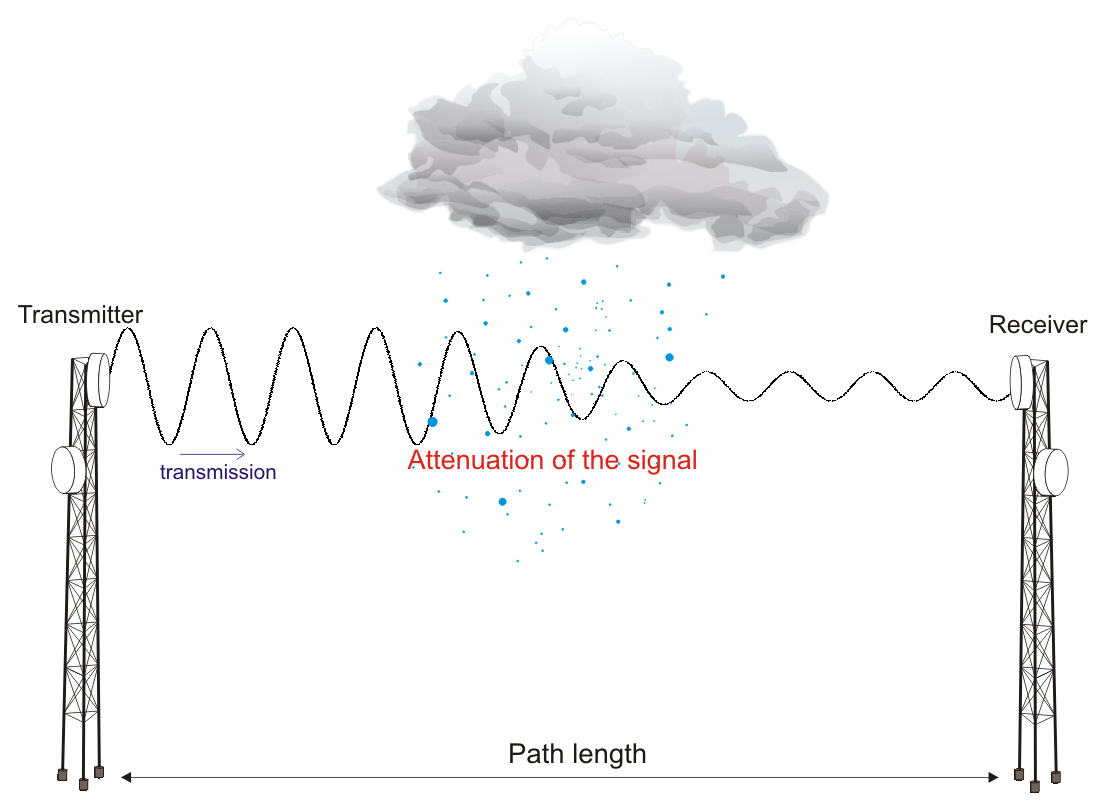
\includegraphics[width=0.7\textwidth]{./img/srazky/microwave_link.png}
    \caption[MV linky]{\centering  Princip odhadu srážek z mikrovlnných spojů }
 \end{figure}   

\subsubsection{Data}
Charakteristika dat z MV spojů je zcela unikátní v oblasti měření srážek. Specifická je především reprezentací hodnoty srážkové intenzity liniově. MV spoje (linie), umožňují odhadovat pouze průměrnou intenzitu srážky v celé délce s poje. Z toho plynou jisté meze této metody. V hustě osídlených lokalitách bývá pravidlem, že i hustota MV spojů je veliká a v takovém případě není tento faktor zcela limitující (Evropa). Oproti tomu při využití MV spojů mimo osídlené lokality je hustota poněkud menší a v případě využití informace o srážce pro transformaci do povodí je nutné provést úvahu o vhodnosti.  Příkladem může být spoj, který vede kolmo přes cílovou lokalitu. V případě že lokalita zasahuje do desetiny délky spoje, je pravděpodobnost toho, že srážka spadla právě do lokality značně nejistá, díky variabilitě srážek a jejich intenzit proměnných až o několik řádů už v rozsahu stovek metrů. 
Oproti tomu pokud bude cílem transformace srážky do povodí, kde spoj bude ležet v celém území povodí, je tento stav ideální. 

Obecně jsou data z MV spojů měřeny v časovém kroku \emph{dt=15} [s], ve výšce cca okolo 70 [m]. Topologie sítě představuje vždy jeden referenční vysílač pro spádové území podrobných vysílačů. Na jednom spoji jsou instalované z pravidla dvě antény. Jsou tedy k dispozici dvoje měření pro stejný prostorový úsek. V ideálním případě jsou dvě antény na stejném prostorovém úseku různých konfigurací (frekvence, polarizace) což umožňuje specifické analýzy.

    
\subsubsection{Princip}
Mikrovlny jsou elektromagnetické vlny o délce v rozpětí od 1 [mm] do 1 [m]. Tomu odpovídá frekvence 0.3  až 300 [GHz]. V oblasti telekomunikací především mobilních operátorů se tohoto typu vln využívá ke komunikaci mezi jednotlivými vysílači a vysílači s mobilními telefony. Pro rekonstrukci srážek se využívá prvního případu, tedy komunikaci mezi vysílači. Tyto mikrovlnné spoje pracují na frekvencích v rozsahu 24-39 [GHz] (Praha). Hlavním zdrojem útlumu tohoto frekvenčního rozsahu jsou dešťové kapky. Jednotlivé spoje se vždy skládají ze dvou vysílačů. Vysílač neustále odesílá MV vlny, které jsou nositelem informace zajímavé především pro telekomunikace. Vedlejším produktem této komunikace je údaj o intenzitě signálu, jehož základní jednotkou je decibel [dB]. Zaznamenat hodnotu intenzity signálu odeslaného a druhým přijímačem přijatého je možné bez dalších instalací hardware. Pomocí fyzikálně-parametrického modelu dle ITU-R\cite{itu} lze vypočítat průměrné srážky na pomyslné linii MV spoje.

\subsubsection{Výpočet srážek}
Vysílané hodnoty intenzit signálu \emph{tx} jednotlivých MV spojů jsou konstantní. Jednotlivé spoje jsou charakterizovány hodnotami:
\begin{itemize}
\item \textbf{Frekvence} \emph{f} rozsahu 24-39 [GHz]
\item \textbf{Polarizace} signálu ve vertikální \emph{V} či horizontální poloze \emph{H}
\item \textbf{Vzdálenost} \emph{L} která je vypočtená v daném souřadnicovém systému v kilometrech[km]
\end{itemize}
Přijaté hodnoty intenzit \emph{rx} jsou nositelem informace o útlumu signálu. Rozdílem vyslané \emph{tx} a přijaté \emph{tx} intenzity dostaneme výsledný útlum \emph{$A_{r}$} v jednotkách decibel[dB].
\begin{equation}
 A_{r}=tx-rx
\end{equation}
Dalším krokem je určení \emph{baseline}, tedy hodnoty \emph{ $A_{0}$ }  ,která představuje konstantní útlum intenzity signálu MV spoje bez vlivu útlumu signálu dešťovými kapkami. Tato konstanta je v jednotkách decibel[dB]. Parametrická konstanta  \emph{$A_{w}$ } je hodnota nadměrného útlumu způsobená mokrou anténou. Z toho plyne výsledný útlum \emph{$A_{m}$ }[dB].
\begin{equation}\label{eq:Ar}
 A_{m}=A_{r}-A_{0}-A_{w}
\end{equation}
 Výsledný útlum je třeba převést na specifický útlum \emph{$\gamma_{R} $} [dB/km] pro danou vzdálenost \emph{L} mezi vysílači MV spojů. 
\begin{equation}
\gamma_{R} =\frac{A_{m}}{L}
\end{equation}
Dle doporučení ITU P.838 \cite{itu} je specifický útlum  \emph{$\gamma_{R} $} a intenzitu srážek  \emph{R} [$mm \cdot h^{-1}$] ve vztahu
\begin{equation}\label{eq:gamma}
\gamma_{R}=kR^{\alpha}
\end{equation}
Koeficienty \emph{k} a \emph{$\alpha$} jsou určeny jakožto funkce frekvencí \emph{f}[GHz] v rozsahu od 1 do 1000[GHz], z následujících rovnic.

\begin{equation}
log_{10}k=\sum_{j=1}^{4} a_{j} exp\left [ -\left ( \frac{log_{10}f-b_{j}}{c_{j}} \right )^{2} \right ]+m {_{k}}log_{10}f+c_{k}
\end{equation}

\begin{equation}
\alpha=\sum_{j=1}^{5} a_{j} exp\left [ -\left ( \frac{log_{10}f-b_{j}}{c_{j}} \right )^{2} \right ]+m{_{\alpha }}log_{10}f+c_{\alpha }
\end{equation}
kde:

\emph{f}: frekvence [GHz]

\emph{$\alpha$}:  dle polarizace \emph{$\alpha_{H}$} nebo \emph{$\alpha_{V}$}

\emph{k}: dle polarizace  \emph{$k_{H}$} nebo \emph{$k_{V}$}

{\raggedright{}Hodnoty pro dané konstanty jsou součástí dokumentu ITU-R \cite{itu}.}
\bigskip

{\raggedright{}Inverzním vztahem rovnice \eqref{eq:gamma} dostaneme výslednou intenzitu srážek \emph{R} [$mm \cdot h^{-1}$]. }


\begin{equation}
R=\left ( \frac{\gamma_{r}}{k} \right )^{\frac{1}{\alpha }}
\end{equation}


\subsubsection{Chyby}
\label{subsec:chyby}
Metoda odhadu srážek je založena na předpokladu, že dešťové kapky tlumí intenzitu signálu. Dešťové kapky nabývají mnoha variací velikosti a tvarů. Signál může být tlumen škálou objektů od vodní páry, jejímž zdrojem je povrch Země, přes mrholení až po velké dešťové kapky. Vztah mezi intenzitou srážek \emph{R} a útlumem \emph{$\gamma_{R} $} je funkcí frekvence, polarizace a rozložení dešťových kapek\acs{DSD} s parametry \emph{a} a \emph{b}. 

Na frekvencích mezi 25 a 40 GHz platí takřka lineární závislost a model je téměř nezávislý na teplotě, rozložení dešťových kapek a empiricky vykazuje chybovost méně než 10\emph{\%}. Na nízkých frekvencích okolo 10 GHz přesahuje chybovost 20\emph{\%}. Přesnost určování srážek výše zmíněným modelem dle ITU P.838 je při těchto nízkých frekvencích mnohem více náchylná na rozložení kapek\acs{DSD}.\cite{dsd} 


\paragraph*{Nejistoty modelu} založeného na vztahu \eqref{eq:Ar} jsou především v závislosti \emph{$\gamma_{A_{m}} $},\emph{$A_{w} $} na rozložení kapek \acs{DSD} podél MV spoje.

\paragraph*{DSD} způsobují nejistoty při určení výsledného útlumu signálu \emph{$\gamma_{A_{m}} $}. Tyto chyby jsou zapříčiněny integrací jednotlivých úseků tlumících signál na linii MV spoje. \cite{mv1}

\paragraph*{Mokré antény}jsou značným zdrojem nejistot. Na vysílačích nejsou antény nijak kryty a při dešti moknou. Na anténách se vytváří tenký film vody, který ovlivňuje výsledný útlum signálu. Vytvoření modelu pro eliminaci tohoto problému se do značné míry podařilo (Schleiss et al., 2013)\cite{wetat}. Součástí výzkumu, pod který tato práce částečně spadá, bude instalace krytu na antény, který by mohl zamezit jejich moknutí. Tato možnost doposud nebyla součástí žádné vědecké práce.

\paragraph*{Určení baseline } \emph{ $A_{0}$ } je jedním z důležitých a nejvíce ovlivňujících činitelů při výpočtu výsledné srážky \emph{R}. Tato hodnota se zcela mění v čase a je závislá na koncentraci vodní páry v atmosféře a scintilaci. Útlum vysílaných a přijímaných vln ovlivňuje také teplota prostředí jímž vlna prochází. Dalším činitelem, který může způsobovat kolísání signálu, je vítr.
Pro určování baseline se využívá různých metod, například \acs{HMM} \cite{comparsinmv}, Retrieval Alghorithms \cite{countryw}. Metody Určení baseline se dají klasifikovat na automatizované a uživatelské. Automatizovaným určováním baseline se myslí především algoritmy, které jsou schopny detekovat, mokré a suché období. Některé tyto algoritmy využívají statistických prostředků a jiné například určují období dešťů pomocí dat ze srážkoměrů \cite{countryw} či radaru. 


\subsection{Porovnání}
Tato podkapitola je zaměřena na shrnutí vlastností jednotlivých metod a jejich porovnání s metodou MV spojů. Hodnocení jednotlivých metod je založeno na kritériích, která jsou pro měření srážek typická.
\begin{itemize}
\item\textbf{Časová spojitost}
\item\textbf{Interval sběru dat}  
\item\textbf{Prostorové rozlišení}
\item\textbf{Disponibilita jednotlivých metod}
\item\textbf{Chyby}
\end{itemize}
V současné době jsou v oblasti hydrometeorologie požadována velmi přesná data ve vysokém prostorovém a časovém rozlišení. Tyto nároky jsou především vytvořeny požadavky hydrologických modelů, jejichž výsledky napomáhají k lepšímu operativnímu řízení odtoku v urbanizovaných územích. Kvalita vstupů dat do těchto modelů je rozhodující pro jejich přesné výsledky, které jsou základem přijímaných opatření vedoucích ke snížením povodňových škod.

\paragraph*{Srážkoměrné sítě} 
tyto požadavky splňují jen částečně. Moderní srážkoměry splňují kritérium schopnosti pokrytí spojité časové řady až v minutových intervalech. Hlavním záporem těchto sítí je nedostatečné pokrytí. Jelikož datovým výstupem těchto sítí jsou bodová data, je zde problém v nedostatečné hustotě pokrytí srážkoměry, která prakticky nemůže být nikdy odstraněna. Prostorová variabilita srážek, kde se jednotlivé mohou řádově lišit už ve stovkách metrů, má za následek zachycení či naopak nezaznamenání lokálních maxim, které jsou ve výsledné plošné rekonstrukci zdrojem nezanedbatelných chyb. Měření moderními srážkoměry může být při správné volbě umístění velmi přesné. Toho se v současnosti využívá jako referenčního indikátoru srážek pro kalibraci radarů, nebo k určování baseline při odhadu srážek MV spoji (\ref{subsec:chyby},Baseline).

\paragraph*{Radary}
jsou současnou nejvíce využívanou metodou umožňující měřené plošné vyjádření srážek. Snímky se pořizují v 5-15 minutových krocích a tento časový interval nelze z fyzikální podstaty radaru zmenšit. To poukazuje na možnou chybovost, jelikož srážky během 5 minut mohou nabývat jiných hodnot až o řád. Mezi kladné vlastnosti radaru bezesporu patří mimo klasické rozlišení v horizontálním směru (plošné) také i měření odrazivosti vertikálních profilů. Tuto vlastnost v rozlišení 1 km pro vertikální a 2 km pro horizontální ostatní metody neumožňují. Prostorové rozlišení je dále možno pozorovat jen pomocí některých meteorologických družic, které skenují Zemi pod sklonem jiným než 90 stupňů. Jejich rozlišení je ale v desítkách jednotek horší. Pro zpřesnění radarových srážek pro potřeby hydrologie je potřeba  adjustace radarů na pozemní srážkoměry. Obecně vzato je výsledné plošné rozlišení radaru pro městské odtokové modely nedostačující.   

\paragraph*{Družice} se z výše zmíněnými metodami nedají zcela korektně porovnávat. Družice na oběžných drahách slouží především k náhledu na chování klimatu. Snímky těchto družic jsou nositelem informací v rozlišení, reflektující spíše obecnou informativní podstatu, např. pohybu front, vývoje cyklónu, globální přehled vývoje počasí, či dlouhodobě- klimatu.
Jednou z výhod rekonstrukce srážek pomocí metody \acs{IR} pásem je poměrně vysoká frekvence záznamu snímků v intervalu 15 minut na jakémkoliv místě na Zemi. Při porovnání s pozemním meteo radarem je slabost této metody ve špatném a u některých družic nulovém detekování vertikálních profilů srážkových mraků, což vede k podceňování výsledných srážkových úhrnů.


\subsubsection{Mikrovlnné spoje}
Metoda odhadu srážek pomocí MV spojů byla předmětem výzkumu už v 80. letech 20. století. Prakticky byla použita až při využití komerčních telekomunikačních spojů v posledním desetiletí. Budoucnost této metody je především v pokrytí  osídlených oblastí, kde je právě přesnost odhadu srážek nejvíce vyžadována. Pokrytí s vývojem mobilních technologií se stále zlepšuje. Data jsou sbírána ve velmi malých intervalech běžně po 15[s]. Při využití rozsáhlých sítí(Praha- stovky MV spojů), umožňuje tato metoda relevantní časoprostorovou informaci o srážce.
 
\paragraph*{Potenciál MV v hydrometeorologii} zasahuje do všech oblastí vědních oborů, kde se využívají srážky jakožto vstupní časové řady. Tato metoda je v současné době spíše vhodná pro lokální využití nežli regionální. Vyplývá to z absence pokrytí sítí mimo osídlené oblasti. 

Jedním z velkých potenciálů této metody je zlepšení přesnosti prostorové informace o srážkách ve vysokém rozlišení. To žádné jiné metody odhadu srážek neumožňují. Výsledky stude\cite{mv2} poukazují na možnosti částečného nahrazení současných metod nebo možnosti vzájemného se doplňování jednotlivých metod, což by patrně vedlo k zlepšení přesnosti měření srážek. 

Jelikož tyto MV spoje operují těsně nad zemským povrchem, vypočtené intenzity by mohly být pomocí nástrojů \acs{GIS}s velkou přesností přiřazovány do jednotlivých subpovodí. To by zpřesnilo vstupy do srážko odtokového modelu a umožnilo lépe modelovat členitá povodí na místě velkých aglomerací.

Možnosti využití MV spojů v oblasti meteorologie nekončí u odhadu srážek. Pomocí MV lze také detekovat pevné částice, sníh, či vodní páry. Tyto možnosti by mohly napomoci k lepšímu pochopení jevů spojených s přívalovými srážkami.\cite{mv2}
\begin{figure}[h!]
    \centering
    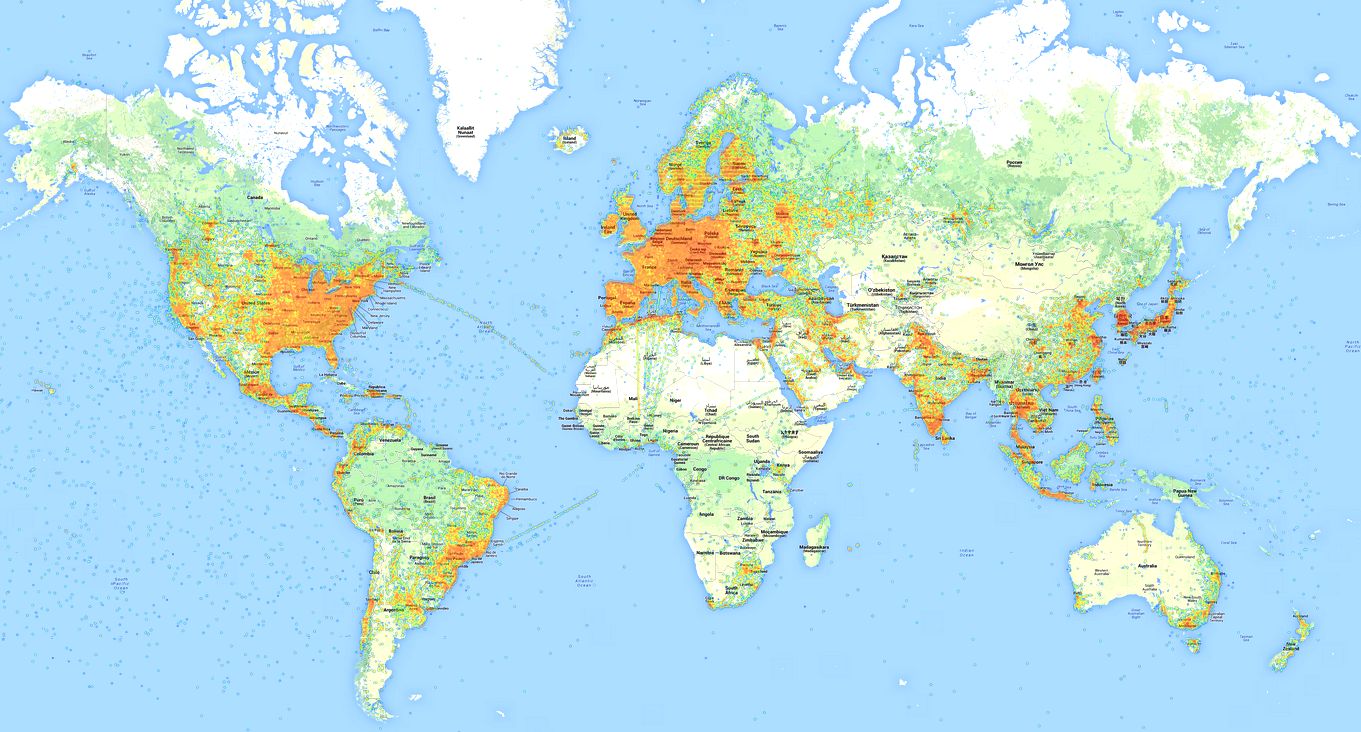
\includegraphics[width=0.8\textwidth]{./img/srazky/opensignalmap.png}
    \caption[Porytí tel. sítí]{\centering Mapa celosvětového pokrytí signálu telekomunikačních mobilních operátorů. Pokrytí je vyjádřeno oranžovou a žlutou barvou. \footnotemark }
 \end{figure}   
\footnotetext{Obrázek byl sejmut z webové aplikace OpenSignal. \url{http://opensignal.com/}}

Velkým potenciálem je takřka nulová finanční náročnost pro sběr dat. Telekomunikační sítě mobilních operátorů jsou v hustěji osídlených částech světa běžné. V rychle se rozvíjejících zemích třetího světa se v průběhu času stanou telekomunikační sítě samozřejmostí a využití metody odhadu srážek by se mohlo stát více dostupnou oproti budování radarů, pozemních stanic, či sítě srážkoměrů.
 
\setcounter{footnote}{1}




\section{Použité technologie}

\subsection{Systém GRASS GIS}
\textbf{GRASS} (Geographic Resources Analysis Support System) GIS \footnotetext{\url{http://grass.osgeo.org/}} je multiplatformní geografický systém, šiřitelný pod všeobecně veřejnou licencí \acs{GNU GPL}. Systém je primárně určený pro správu 2D/3D rastrových a vektorových geodat, jejich zpracování, analýzu a vizualizaci. K těmto účelům knihovna GRASS GIS disponuje několika stovkami modulů, které jsou současní stabilních verzí. Mimo to je volně dostupných mnoho jiných modulů, které jsou vyvíjeny uživateli v rámci GRASS \textit{AddOns} a mohou se stát součástí stabilních vývojových verzí GRASS. 

GRASS GIS je na poli GIS software zcela unikátní a to především díky svému rozsahu, čemuž vděčí především dobrovolným vývojářům z komunity GRASS po celém světě, kteří tento dlouholetý projekt vyvíjí. Za jeho kvalitu jsou důkazem uživatelé mezinárodního charakteru jako \textit{NOAA}\footnote{\url{http://www.noaa.gov/}} či \textit{NASA}\footnote{\url{http://www.nasa.gov/}}. 

\begin{figure}[h!]
    \centering
    
\includegraphics[width=0.3\textwidth]{./img/grass/grasslogo.png}
    \caption[Logo GRASS]{\centering Logo GRASS GIS vydané symbolicky k 30. výročí od založení projektu. \footnotemark }
 \end{figure}   
\footnotetext{\url{http://grass.osgeo.org/uploads/images/30-years-grass-gis-logo-black-300px.png}}


\subsubsection*{Historie}
Vývojová linie GRASS GIS je stálá od poloviny osmdesátých let minulého století, kde byl vyvinut primárně pro americkou armádu, která jej využívala pro územní správu a plánování. Během 90. let se postupně na vývoji projektu podíleli americké federální agentury, univerzity a soukromé společnosti. Hlavní vývoj projektu byl řízen z výzkumných laboratoří (USA-CERL\footnotetext{\url{http://www.cecer.army.mil/}}) Champaign, Illinois.\cite{grasshist}.
Mezníkem historie GRASSu byl rok 1995, ve kterém se laboratoře CERL zřekli tohoto projektu, čehož   následkem bylo přesun vývoje na akademickou půdu. Rok před začátkem nového tisíciletí byla vydána první verze pod licencí GNU GPL, pod kterou je vyvíjen dodnes. V letech 2008 se GRASS GIS zařadil do nadace \acs{OSGeo}, pod kterou spadá mnoho významných volně šiřitelných geografických projektů.\footnotetext{\url{http://www.osgeo.org/}}. Letošním rokem oslavil GRASS dlouhých 30 let vývoje, které zaštítil vydáním verze \textit{GRASS GIS 7.0.0 beta1}.\footnotetext{url{http://grass.osgeo.org/news/32/56/GRASS-GIS-7-0-0-beta1/}}

\subsubsection*{Základní terminologické pojmy}
\label{subsubsec:grassterminologie}
Hlavním cílem této sekce je představit základní filosofii uživatelského rozhraní systému GRASS GIS.
\paragraph*{Data} ke kterým GRASS přistupuje, jsou definována  pevně stanovenou  adresářovou  strukturou. Pro práci v tomto systému, je prvně zapotřebí definovat trojici nastavení. V grafickém rozhraní GRASS \acs{wxGUI} je implementován průvodce nastaveni pro jednotlivými kroky 

\begin{enumerate}
\item \textbf{Database} v prostředí GRASS je stanovena proměnou \texttt{\$GISBASE}. Jedná se o standardní adresář umístěny na disku, který je pojmenován (\textit{grassdata}). V tomto adresáři jsou uloženy veškerá uživatelská data mimo externě připojené databáze (\textit{např. PostgreSQL, MySQL }).

\item \textbf{Lokace} je adresář umístěný v souborové databance. Lokace je definována proměnou   \texttt{\$LOCATION\_NAME}
a obsahuje data, která nesou informace o souřadnicovém systému a velikosti zájmového území. Pro nastavení lokace je v grafickém rozhraní průvodce nastavením lokace (\textit{Location wizard}), kde je možné zvolit souřadnicový systém pomocí možností.
\begin{itemize}
\item seznam jednotlivých obecně známých projekcí 
\item zadáním unikátního kódu z databáze \acs{EPSG}. \footnote{\url{http://www.epsg-registry.org/}}
\item načtením externích georeferencovaných dat
\item definováním parametrů projekce s využitím pravidel PROJ.4\footnote{\url{http://trac.osgeo.org/proj/}}
\item pomocí \ac{WKT} souboru .prj, který je součástí shapefile jako doplňkový.
\end{itemize}

\item \textbf{Mapset} definovaný proměnou \texttt{\$MAPSET} představují jakýsi profil uživatele, či profil ucelených analýz  v dané lokaci. Každá lokace musí obsahovat mapset, který má unikátní název \texttt{PERMANENT}. Do tohoto mapsetu se z pravidla ukládají vstupní data, ke kterým se z ostatních pracovních mapsetů přistupuje.
\end{enumerate}



\paragraph*{Modul} je nedílnou součástí navržené architektury tohoto geoinformačního systému. Volba implementace pomocí jednotlivých modulů pochází z doby, kdy vypočtení technika byla v počátcích a šetrné využití operační paměti a procesorového výkonu bylo nezbytností. Jádro systému je napsáno procedurálně v jazyce C k němuž jsou  jednotlivé funkcionality integrovány pomoci \acs{API}, které je v jazyce C a Python. Funkcionality-moduly jsou logicky rozděleny do kategorií, podle účelu jejich využití.

\begin{table}[h]
\centering
\begin{tabular}{|cccccccc|}
\hline
db. & d. & g. & i. & ps. & r3. & r. & v. \\
\hline \hline
database & display & general & imagery & postscript & 3D raster & raster & vector \\ \hline
\end{tabular}
\caption{Přehled jednotlivých skupin modulů a jejich prefixů v GRASS GIS}
\label{tab:module}
\end{table}


Nyní také nově v \textit{GRASS 7} moduly \textit{Temporal GRASS} s prefixem \texttt{t.} Jednotlivé moduly se spouštějí pomocí příkazové řádky a nebo v grafickém rozhraní \textit{wxGUI} . Rozhraní modulů umožňuje uživatelský vstup pomocí přepínačů a parametrů např. \texttt{r.mwprecip -p database=letnany}. Parametry se dělí na povinné (\texttt{required}) a volitelné (\texttt{optional}). V modulech jsou také globální přepínače, které jsou pro všechny moduly definovány jednotně. Mezi nejčastěji využívané patří \texttt{--help}, který do terminálu vypíše veškeré informace o vstupních parametrech včetně jejich  popisu.

\subsubsection*{GRASS a Python}
GRASS GIS v současné době podporuje dva přístupy k volání funkcionalit GRASSu z prostředí Python.
\paragraph*{Python Scripting Library} je variantou API, které tvoří Python podporu pro funkcionality GRASS. Princip této knihovny spočívá v zadávání příkazu v analogickém formátu, jako je formát pro spouštění jednotlivých modulů přímo v GRASS.
\paragraph*{pyGRASS} je objektově orientovaná API knihovna. Výhoda tohoto API spočívá ve možnosti přiřazování výsledků z volaných GRASS funkcionalit v podobě objektů. Tento přístup je současným trendům více odpovídající.

\subsection{PostgreSQL}
PostgreSQL\footnote{\url{http://www.postgresql.org/}} je open-source projekt, který vznikl v roce 1986. Tento projekt je dnes celosvětově uznávaný, čehož důkazem je využití systému ve světových projektech jako \textit{SourceForge}\footnote{\url{http://sourceforge.net/}}, \textit{Debian}\footnote{\url{http://www.debian.org/}} či \textit{Open Street Map}\footnote{\url{http://www.openstreetmap.org\#map=15/49.9503/14.5322}}. Kvalita systému a rozsáhlá dokumentace je především dílem komunity dobrovolníků, díky kterým je PostgreSQL schopno konkurovat i proprietárním databázovým systémům. Tomu také mimo jiné přispívá fakt, že se řadí mezi multiplatformní systémy.\cite{postgre}

\begin{figure}[h!]
    \centering
    
\includegraphics[width=0.2\textwidth]{./img/implementace/postgresql.png}
    \caption[Logo PostgreSQL]{\centering Logo PostgreSQL }
 \end{figure}   


\subsubsection{Princip databáze PostgreSQL}
\paragraph*{Architektura}
PostgreSQL je \ac{ORDBMS} tedy systém relační databáze doplněný o objektově orientovaný model. Funguje na principu klient-server, kde každý klient je obsluhován samostatným procesem, který se stará o zpracování dotazu. Tedy \textit{host} server se skládá ze dvou částí: \textit{postmaster} a \textit{postgres}.  Když klient odešle požadavek k přístupu k databázi na server, \textit{postmaster} na serveru založí nový proces \textit{postgres} a ten přímo komunikuje s klientem. Z toho plyne že proces \textit{postmaster} musí nepřetržitě běžet, oproti tomu  proces \textit{postgres} začne a skončí na příkaz klienta. 


\paragraph*{Zpracování dotazu}
Dotazy se dělí podle jejich typu na optimalizované a neoptimalizované. Do skupiny optimalizovaných spadají příkazy z \ac{DML}. Ty jsou charakteristické právě pohybem/manipulací s daty. Patří mezi ně \texttt{SELECT}, \texttt{INSERT}, \texttt{UPDATE}, \texttt{DELETE} a další méně využívané. \acs{DDL}  představuje skupinu neoptimalizovaných dotazů, což plyne z jejich funkčnosti. Patří mezi ně především \texttt{CREATE}, \texttt{ALTER}, \texttt{DROP} a další. \cite{bares}


\begin{table}[h]
   \centering
\begin{tabular}{|ccll|}
\hline
definice & optm* & příkaz & popis \\ \hline \hline
\multirow{4}{*}{DML} & \multirow{4}{*}{$+$} & SELECT & vybírá data z databáze \\
 &  & INSERT & vkládá do databáze nová data. \\
 &  & UPDATE & editace data v databáz \\
 &  & DELETE & odstraňuje data \\ \hline
\multirow{4}{*}{DDL} & \multirow{4}{*}{$-$} & CREATE & vytváření nových objektů \\
 &  & ALETER & změny existujících objektů \\
 &  & DROP & odstraňování objektů \\
 &  & TRUNCATE & mazání všech záznamů z tabulky \\ \hline
\end{tabular}

\caption{Zařazení a popis SQL příkazu do kategorii.
*( ne/optimalizovaných )}
\label{tab:prikazy}
\end{table}


\begin{description}
\item[Parser]zastupuje funkci validátoru syntaxe. Zkontroluje správnou syntaxi vstupu a pokud je platná, transformuje příkaz na stromovou strukturu (\textit{query tree}). Součástí kontroly syntaxe je i testování existence jednotlivých výrazů, tabulek, schémat, atributů a dalších.

\item[Traffic Cop] identifikuje dotaz do výše zmíněných kategorií, tedy optimalizované\-/neoptimalizované.

\item[Utility Commands] je proces, který zpracovává jednoduché dotazy ze skupiny neoptimalizovaných. Z podstaty věci tyto příkazy nelze  optimalizovat.

\item[Planner/rewriter] také optimalizátor má za úkol vygenerovat optimální exekuční řešení. Pro vyhledání optimální cesty se využívá síťových analýz, kde jednotlivé cesty jsou  ohodnoceny a algoritmus vybere obecně tu nevýhodnější.

\item[Exekutor] pracuje pouze s \acs{DML}. Obdrží od výše zmíněného \textit{planneru} plán nejvýhodnější cesty a začne daný strom procesů zpracovávat od horního uzle.
\end{description}


  
\begin{figure}[h!]
    \centering
    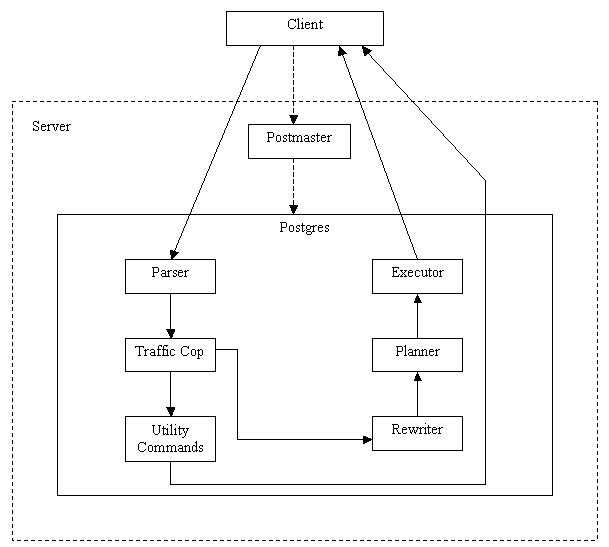
\includegraphics[width=0.6\textwidth]{./img/implementace/postgremodel1.jpg}
    \caption[Dotaz PostgreSQL]{\centering  Zpracování dotazu \footnotemark}
 \end{figure}   
\footnotetext{\url{http://reshmaparveen.blogspot.cz/2009/12/normal-0-false-false-false.html}}




\subsubsection{Vlastnosti}
PostgreSQL je systém relační databáze doplněný o objektově orientovaný model. Ten je specifikován v rozšíření standardu SQL3 z roku 1999\cite{sql1999}. Objektový model podporuje objekty, třídy a dědičnost v databázových schématech. Objektově-relační systém pro zprávu databáze  poskytuje střední cestu mezi relační a plně objektově orientovanou databází. To je vhodné v možnosti vytváření vlastních datových typů a metod, které umožňují vyšší míry abstrakce. Nechybí podpora implementace vlastních procedur buď s využitím vlastního jazyka PL/pgSQL nebo využít externí podpory C/C$++$ (knihovny libpq a libpq$++$), Python (PyGreSQL), Perl (pgsql\_perl5).


\paragraph{Objekty} umožňují vytvoření nových datových typů. Konverze, přetypováním, indexy, funkce, agregační funkce, operátory a další.  
\paragraph*{Funkce} umožňují spouštění bloků kódu, které mohou být jak v nativním jazyce PL/pgSQL, tak i v ostatních výše zmíněných podporách. Funkce po spuštění vracejí výsledek v řádcích, tedy tabulkou, kterou je možné využít k dalším příkazům. Možnost je vytvoření vlastních funkcí, či využití funkci z nativní knihovny PostgreSQL nebo také funkce externě funkce z přidaných extenzí (\texttt{EXTENSION}).
\paragraph*{Indexy} PostgreSQL umožňuje vytvářet pomocí algoritmu \textit{B-tree}, \textit{hash}, \textit{GiSTm} a \textit{GIN} \footnote{\url{http://www.postgresql.org/docs/9.1/static/sql-createindex.html}}, nebo lze vytvářet i vlastní. Princip indexu spočívá ve vytvoření specifického sloupce v tabulce, jehož jediný úkol je optimalizovat prohledávání daného sloupce. 
\paragraph*{Pravidla} umožňují nad jednotlivými tabulkami nebo pomocí \texttt{SELECT} vytvářet náhledy (\texttt{VIEW}). Principiálně jde o virtuální tabulky, které jsou logicky odkazují na vyprané sloupce v jiných tabulkách. V \textit{PostgreSQL 9.3 } jsou nově implementované materializované pohledy (\texttt{MATERIALIZED VIEW}), které představují  jak charakteristiky tabulky  tak i pohledu. Data materializovaných pohledů jsou fyzicky uloženy na disku. Jejich hlavní výhoda spočívá v možnosti obnovení (\texttt{REFRESH}), čímž doje k obnovení tabulky na základě logických vazeb z vytvoření.
\paragraph*{Triggery} (spouštěče) mají funkcionalitu v podobě kontroly událostí, na které reagují podle své definice. Například při vytvoření nového záznamu provedou definovanou operaci v databázi. 
\paragraph*{Datové typy} definují druh nebo význam hodnot. V PostgreSQL je široká škála datových formátu. Specifickými pro tuto práci jsou: numerické, časové, logické, řadící (enumerate) a geometrické typy.

\subsection{Extenze PostGIS}
PostGIS\footnote{\url{http://postgis.net/}} je open-source rozšířením \texttt{EXTENSION} databáze PostgeSQL o podporu geografických objektů. Jde tedy o velice vhodný   nástroj pro využití v GIS. PostGIS implementuje specifikaci \textit{Simple Features for SQL}\footnote{\url{http://www.opengeospatial.org/standards/sfs} } konsorcia \acs{OGC}, která v současné době plní funkci standardizační organizace pro geoprostorová data. PostGIS je 2D/3D  vektorovou databázovou nadstavbou, vedle které je i extenze PostGIS Raster. 

  
\begin{figure}[h!]
    \centering
    
\includegraphics[width=0.2\textwidth]{./img/implementace/postgis.png}
    \caption[Logo PostGIS]{\centering  Logo PostGIS \footnotemark}
 \end{figure}   
\footnotetext{\url{http://postgis.net/docs/manual-2.1/}}

\paragraph*{Geometrický model} 
Prostorový model je založen na specifikaci \acs{OGC} \textit{Simple Feature}, z toho plyne že model nepodporuje geometrickou topologii. OGC definuje jednotlivé operace mezi standardem SQL a prostorovými daty. Souřadnice jednotlivých objektů jsou ukládány v tabulkách, kde každá tabulka je specifická jedním typem geometrie (bod, linie, polygon atd.) a referenčním prostorovým systémem. Souřadnice jsou ukládány ve standardu \acs{WKT}. Spolu s  metadaty o geometrickém prvku jsou ukládány ve sloupci \texttt{geometry}, který je  nositelem informací o geometrickém typu a referenčním systému.\cite{postgis}

\begin{figure}[h!]
    \centering
    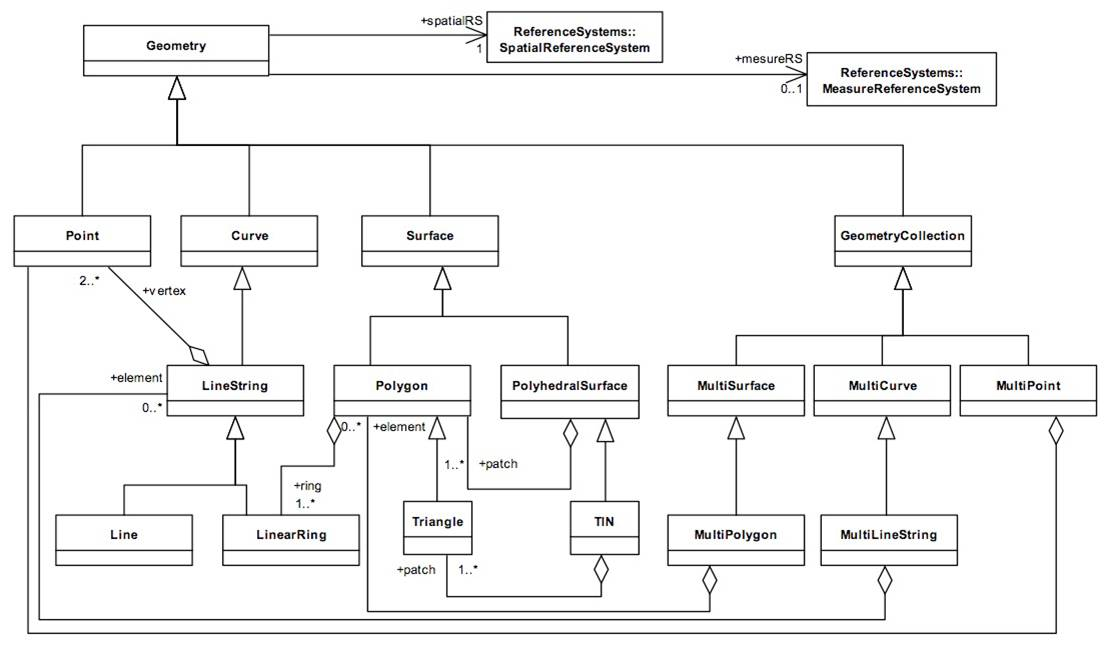
\includegraphics[width=1\textwidth]{./img/implementace/ogc1.jpg}
    \caption[Model PostGIS]{\centering Jednotlivé základní geometrické objekty jsou agregovány do složitějších tzv. Multi Obejct.     \footnotemark}
 \end{figure}   
\footnotetext{\url{http://www.opengeospatial.org/standards/sfs}}

\paragraph*{Souřadnicový systém} \texttt{SPATIAL\_REF\_SYS} je v PostGIS  definován v samostatných tabulkách. Obecně známé referenční systémy jsou již předdefinované, ostatní se dají dodatečně definovat a upravovat.

\begin{verbatim}
CREATE TABLE spatial_ref_sys (
  srid       INTEGER NOT NULL PRIMARY KEY,
  auth_name  VARCHAR(256),
  auth_srid  INTEGER,
  srtext     VARCHAR(2048),
  proj4text  VARCHAR(2048)
)
\end{verbatim}

Souřadnicové systémy a projekce jsou charakterizovány unikátním kódem \texttt{\acs{SRID}}, který je všeobecným standardem v GIS. Pro konverze mezi jednotlivými systémy slouží funkce \texttt{ST\_Transform}.\footnote{\url{http://postgis.org/docs/ST_Transform.html}}


\paragraph*{Geometrie} \texttt{geometry} je datovým typem, který představuje geometrickou složku objektu.  Charakteristika tohoto datového typu je dána standardem \textit{Simple Features} ve formátu \acs{WKT}.
Sloupec s geometrií je definován pomocí parametrů, které nastavují obecné a geometrické  specifika: název, \textbf{typ}, souřadnicový systém a další.
Pro definování \textbf{typu} objektu jsou k vytvořeny funkce \texttt{ST\_Make* }, kde \texttt{*} jsou níže uvedené typy standardu \textit{Simple Fetures}. 


\begin{verbatim}
POINT(0 0)                                               
LINESTRING(0 0,1 1,1 2)                                       
POLYGON((0 0,4 0,4 4,0 4,0 0),(1 1, 2 1, 2 2, 1 2,1 1))          
MULTIPOINT(0 0,1 2)                                              
MULTILINESTRING((0 0,1 1,1 2),(2 3,3 2,5 4))                       
MULTIPOLYGON(((0 0,4 0,4 4),(1 1,2 1,2 2)), ((-1 -1,-1 -2,-2 -2,))) 
GEOMETRYCOLLECTIONM(POINTM(2 3),LINESTRINGM(2 3,3 4))                
\end{verbatim}

\paragraph*{Funkce} jsou  v této nadstavbě zaměřeny na operace s geometrii. Veškeré funkce mají prefix \texttt{ST\_} (\textit{spatial type}). Část z nich je funkčností analogicky odvozena z nástrojů GIS. Funkce jsou podle svého účelu roztříděny do kategorii. Níže jsou demonstrovány  kategorie a nejzákladnější  funkce.
\begin{description}
\item[Měřičské] funkce jsou typické prostorovými výpočty; plocha \texttt{ST\_Area}, vzdálenost \texttt{ST\_distance}, vzdálenost na elipsoidu \texttt{ST\_length\_spheroid} a další. 

\item[Geometrické konstruktory] slouží k vytváření geometrie podle \textit{Simple Feature}; vytvoření bodu \texttt{ST\_MakePoint}, linie \texttt{ST\_MakeLine}, polygonu \texttt{ST\_MakePolygon} a dalších.

\item[Analytické] funkce jsou v PostGIS implementovány dle standartu SQL-MM  vyplývající z ISO99, standard o multimédiích. 				\cite{sqlmm}. V této kategorii jsou funkce typické prostředí GIS. Mezi ně například patří: buffer \texttt{ST\_Buffer}, validita geometrie \texttt{ST\_IsValid}, sjednocení \texttt{ST\_Union}.

\item[Konverze] umožňují transformace mezi referenčními system. Dále pak umožňují oboustrannou konverzi mezi binárními a textovými formáty. Například do \acs{WKT} 

\begin{verbatim}
SELECT  ST_AsEWKT (geom) FROM link
.......
.......
"SRID=4326;LINESTRING(14.4533605575562 50.0689735412598,
                      14.4754581451416 50.0387687683105)"
\end{verbatim}

\item[Agregační] funkce PostGIS jsou z principu  stejné jako ve standardu SQL (průměr, max, min) s rozdílem, že jsou zaměřeny na geometrická data. Příkladem je funkce pro sjednocení \texttt{ST\_Union}.
\end{description}












\setcounter{footnote}{1}
\section{Plošné interpolace }
\label{sec:plostneinterpolace}
Plošné interpolace slouží k odhadu hodnot v prostoru, jež jsou pomyslně ohraničeny výchozími daty, které se uvažují jako referenční. Nutnost odhadovat hodnoty má logickou návaznost na problematiku sběru dat.  Podobně tomu je i v oblasti hydrometeorologie\ref{subsec:11}. Možnou variantou interpolací v GIS systémech je datový vstup reprezentovaný bodovým polem (vektor) a výstup v podobě rastru (grid). Interpolace se také využívají k převzorkování rastrů do jiného rozlišení.

Další metodou, která si je interpolaci blízká, je extrapolace. Extrapolací je myšlen postup, kdy jsou odhadovány data mimo prostorovou doménu referenčních bodů. Extrapolace oproti interpolaci je typicky méně přesná.

Pochopení základních  principů, na  kterých jsou interpolace založené, může přispět k dosažení kvalitních výsledků. Důležité je především znát funkcionalitu volitelných parametrů u jednotlivých metod, které je potřebné v nástrojích GIS nastavit. Následující text je zaměřen na nativně implementované interpolační metody, kterými disponuje systém GRASS GIS pro vektorová bodová data. 


\subsection{Metody}
Jednotlivé interpolační metody se obecně mohou kategorizovat do dvou hlavních skupina, a to na deterministické a geostatistické. 
Deterministické metody jsou charakteristické tím, že pro odhad neznámých využívají neměnnou matematickou funkci. Jinak řečeno oproti geostaticické metodě, nevyužívají pokročilejších statistických metod.

V systému GRASS GIS je nativně implementována čtveřice typů interpolací, pro které jsou vstupem  bodová vektorová data. Všechny čtyři se řadí do skupiny deterministických metod.

Do geostatistických metod bychom mohli zařadit metodu kriging, která je v GRASS GIS podporována externě ze statistického systému \textit{R Project} \footnote{\url{http://www.r-project.org/}}.



\begin{table}[h]
\centering
\begin{tabular}{|ll|}
\hline
interpolace & GRASS modul \\ \hline\hline
Bilinear spline & \multirow{2}{*}{v.surf.bspline} \\
Bicubic spline &  \\
Regularized spline tension & v.surf.rst \\
IDW & v.surf.idw \\ \hline
\end{tabular}
\caption{Přehled vhodných metod v GRASS GIS}
\label{my-label}
\end{table}


\paragraph{Bilineární interpolace} Princip bilineární interpolace je v rozšíření lineární interpolace na funkci dvou proměnných. Každá buňka rastru je definována pomocí bilineární funkce. Interpolace je výpočetně triviální a využívá se často k převzorkování.

Název této interpolace je poněkud zavádějící. Odhad hledaného bodu \emph{P} je definován kvadratickou funkcí $f(x,y)$. 

Postup je takový, že  se nejdříve nad danou množinou bodů provede lineární interpolace z jedné strany rastru na druhou(osa-\emph{x}), tím získáme bod \emph{A} a \emph{B}. Z těchto bodů se  pak ve směru kolmém (osa \emph{y}) interpoluje bod P. Volba pořadí jednotlivých směru je volná. Nejprve tedy dostaneme lineární koeficienty pro $f(x)$ ze kterých  následně vypočteme lineární interpolací koeficienty  pro $f(y)$. Tím dostaneme požadovaný odhad $f(x,y)$  pro bod \emph{P}

\begin{figure}[h!]
    \centering
    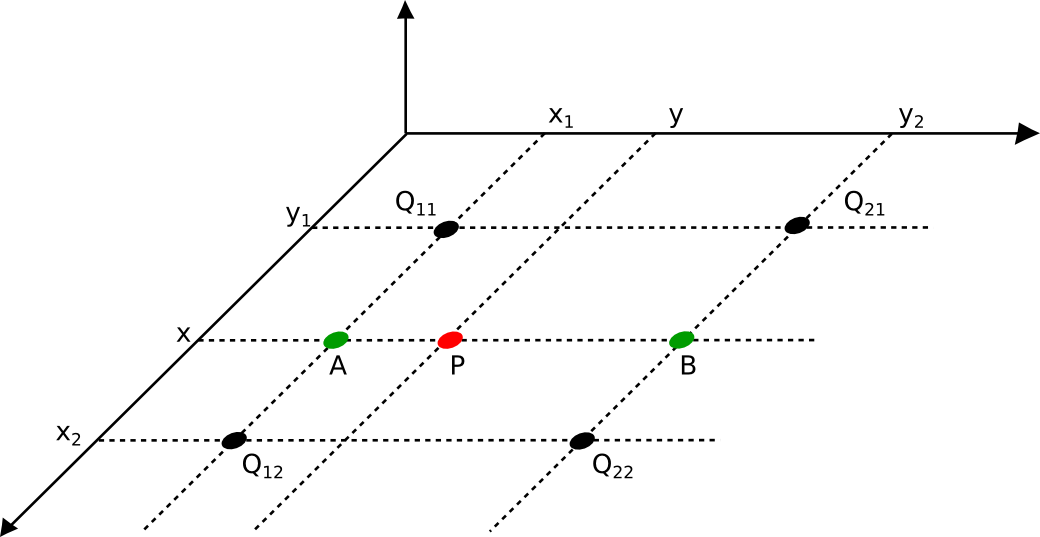
\includegraphics[width=0.65\textwidth]{./img/interpolace/bilinear.png}
    \caption[Bilinear interpol.]{\centering  Zobrazení principu bilineární interpolace \footnotemark}
 \end{figure}   
\footnotetext{\url{http://postgis.net/docs/manual-2.1/}}



\paragraph{Bikubická spline} iterpolace je rozšíření kubické interpolace o druhý rozměr. Principem je podobná bilineární interpolaci s rozdílem, že k výpočtům odhadovaných bodu využívá kubické spline interpolace.  Využití \textit{spline} metody zajišťuje to, že první a druhá parciální derivace polynomu pro odhad koeficientů je spojitá. Oproti bilineární interpolaci je tak výsledný rastr vyhlazenější a celkový výsledek je přesnější. \cite{bicubic}



\paragraph*{Inverse Distance Weighting}
\acs{IDW} využívá k odhadu bodu \emph{P} základního statistického prvku. Určovaný bod \emph{P}  je počítán jako vážený průměr hodnot  bodů známých bodů $Q_{i}$.  Myšlenka je založena na předpokladu, že sobě bližší body jsou si hodnotou více podobné, než ty co jsou od sebe vzdálené. Váhy se tedy počítají inverzně ze vzdáleností $d_{0,i}$. Pro nastavení citlivosti interpolace slouží parametr \emph{p}, který je exponentem  vzdálenosti $d_{0,i}$. \cite{spatialinter}

\begin{equation}
P_{i}=\frac{\frac{1}{d_{0,i}^{p}}}{\sum_{i=1}^{n}\frac{1}{d_{0,i}^{p}}}
\end{equation}

Z tohoto vztahu plyne, že s rostoucím koeficientem \emph{p} mají jednotlivé  body $Q_{i}$ rozdílnější váhy. Při volbě $p=0$ se výsledný bod \emph{P} vypočte jako aritmetický průměr z všech bodů $Q_{i}$.

\paragraph*{Regularized spline with tension}

Metoda Regularized spline with tension odhaduje neznámé hodnoty pomocí spline křivky, která je definována jako funkce, která prochází měřenými body a má minimální křivost. Pro názornost bývá ve výukových textech uveden příklad: Spline funkce si lze představit jakožto imitaci tenkého povrchu, který prochází všemi danými body a zároveň je tento povrch minimálně zakřiven. Tenzi, neboli napětí si lze představit jako prohýbaní, které by vzniklo při nahrazení povrchu různými materiály od elastické gumy po tlustý plech.

Výhody RST interpolace jsou v možnosti kontroly parametrů:

\begin{itemize}
\item napětí
\item vyhlazení
\item anisotropie - rotace
\end{itemize}
Funkce spline je definována vztahem:

\begin{equation}
S(x)=T(x)+\sum_{j=1}^{n}\lambda_{i}R(r,r_{j})
\end{equation}

kde $T(x)$ je trend funkce, $\lambda_{j}$ jsou neznámé koeficienty daných bodů, které se řeší soustavou lineárních rovnic. Funkce $R(r,r_{j})$ je radiální funkcí explicitně závislé na koeficientu vyhlazení. \cite{RST}


\begin{figure}[h!]
    \centering
    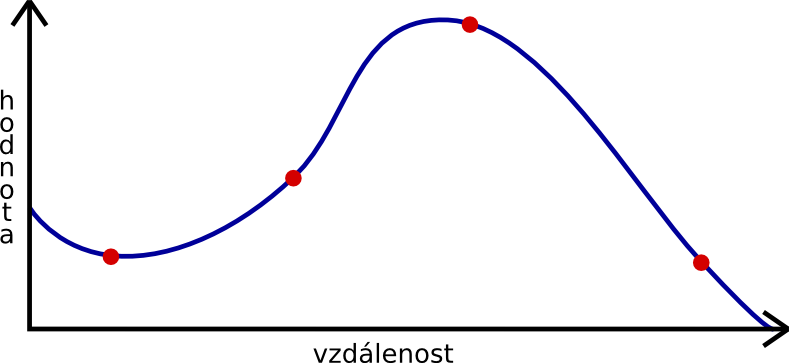
\includegraphics[width=0.65\textwidth]{./img/interpolace/spline.png}
    \caption[Spline interpol.]{\centering  Křivka spline prochází všemi body pod minimálním zakřivením }
 \end{figure}   


\subsubsection{RMS}
Jednou z možných charakteristik přesnosti interpolačních metod je střední kvadratická chyba (RMS error). Tato chyba je ovlivněna jak vhodností zvolené interpolační metody, tak jejím nastavením. Chyba RMS se vypočte pomocí porovnání vstupních hodnot s interpolovanými hodnotami v místech vstupních bodů. Některé metody jsou charakteristické tím, že jejich interpolované hodnoty jsou ve známých bodech stejné jako vstupní (IDW). V takovém případě se využívá jiných metod. Charakteristika RMS může mít veliký podíl při volbě konečné konfigurace dané interpolace a v literatuře bývá uváděna jako hlavní ukazatel přesnosti při porovnání jednotlivých metod.


















\newpage
\setcounter{footnote}{1}
\section{Časoprostorové analýzy}
Hlavní účelem GIS systému je  vytvoření informačního systému, který umožňuje získávání, ukládání, analýzu a vizualizaci dat, která mají prostorový rozsah povrchu Země. Všeobecně je hlavním cílem vytvoření operačních modelů založených na reálném světě. Pro modelování některých reálných jevů je nedílnou součástí časová složka. Z náhledu na historický vývoj většiny GIS software vyplývá, že primární zaměření vývoje bylo nejvíce zaměřeno na práci s prostorovými daty, nikoli však časoprostorovými. Software pro zpracování  časoprostorových dat byl z pravidla vyvíjen samostatně, mimo systémy GIS. Nicméně v poslední dekádě přestal být z velké části tento fakt pravdivý.\cite{geospatialanal} Systém GRASS nyní v nové verzi \textit{GRASS GIS 7 } obsahuje kompletně nově navržený balíček modulů TGRASS \footnote{\url{http://grass.osgeo.org/grass70/manuals/temporalintro.html}}, který integruje do tohoto GIS systému časový rozměr.

Hlavním cílem teoretické části je představení časoprostorových datových modelů s primárním zaměřením na model, který je implementován v  modulech TGRASS. S využitím TGRASS budou v praktické části definovány vhodné funkce pro analýzu zrekonstruovaných srážek pomocí vlastního modulu \textit{r.mwprecip}. K teoretické části byla jako primární zdroj využita kniha (\textit{Geographical information system vol.2})\cite{gistemporal}


\subsection{Terminologie}
\label{subsec:terminologie}
V rámci této podkapitoly jsou čtenáři přiblíženy terminologické výrazy z problematiky časoprostorových GIS. Hlavním zdrojem pro definice byla publikace \cite{pelekis}
\begin{description}
\item[Reprezentace času] Jednotlivé stavy geodat jsou odkazovány k  časovým okamžikům dvěma způsoby a to relativně  (\textit{dny, roky, minuty})  či absolutně (\textit{1990-30-06 1:35:59}). Možností relativní reprezentace je vyjádření času záporně (\textit{-rok}). Další reprezentace je vyjádřena pomocí klasického dělení časů (\textit {před- minulý, teď- současný, po- budoucí}).

\item[Diskrétně časový model] je takový model, kde se proměnné, tedy geodata  mění skokově. Geodata jednotlivých okamžiků na sebe navazují podle dostupného či zvoleného časového rozlišení(granularity). Vhodným příkladem je sčítání lidu v daném intervalu

\item[Kontinuální/spojitý časový model] je charakteristický velice jemným časovým rozlišením. Příkladem jsou data získaná ze seismografu, či kontinuálního měření průtoku řek.

\item[Časová topologie] je termín, který podstatou definice odpovídá  termínu prostorová topologie, s rozdílem že se jedná mimo prostorový rozměr i o časový. Časová topologie geodat definuje vztahy mezi jednotlivými okamžiky daných objektů v datasetu.

\item[Granularita] je ve spojení s časoprostorovými daty definován jako velikost základního časového intervalu na dělené časové ose. Tento bod definuje počátek časové osy, která je dělena v daném rozlišení (zrnitosti). 
\end{description}

\subsection{Časoprostorové modely}

Časoprostorové modely se liší v jednotlivém pojetí vztahů, které propojují časovou složku s prostorovými daty. Současný vývoj a specifické nároky vědních oborů vytvořil poměrně velikou škálu časoprostorových modelů \cite{pelekis}, které jsou často sjednoceny  základní myšlenkou a liší se pouze specificky. Níže jsou přiblíženy principy základních modelů se zaměřením na \textit{Snapshot model}, který je také časoprostorovým modelem v TGRASS.

\subsubsection*{Snapshot model}
Jedná se o jeden z nejrozšířenějších a nejednodušších časoprostorových modelů. U tohoto modelu je začlenění časových složek aplikováno pomocí relačního modelu, který je charakteristický relačními tabulkami, tedy členění daných vektorových či rastrových rámců do jednotlivých časových vrstev/tabulek. 

\begin{figure}[h!]
    \centering
    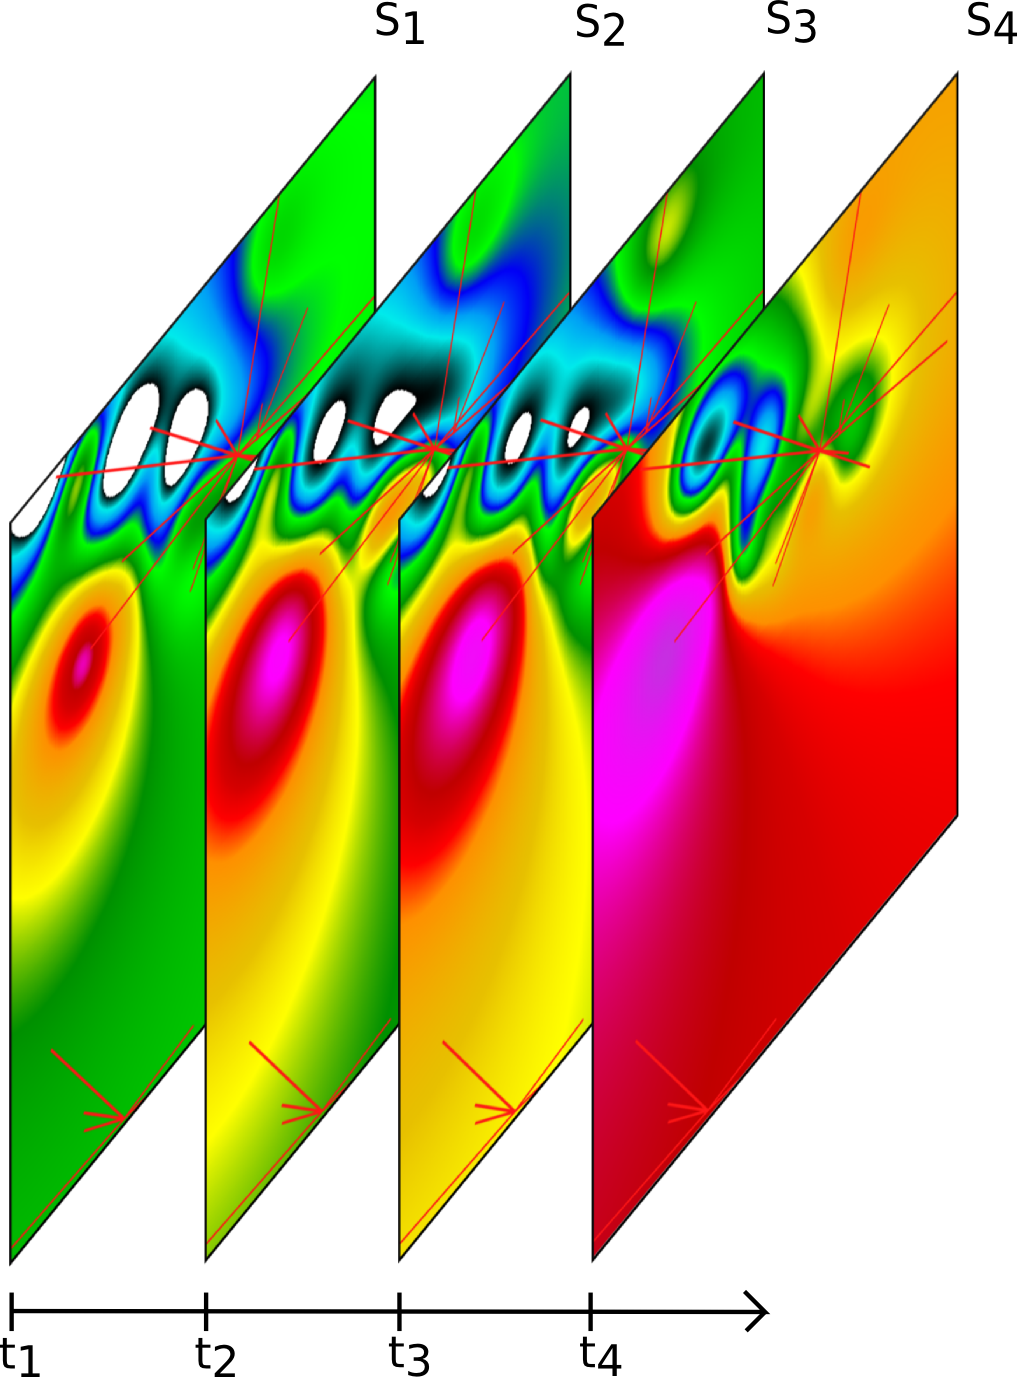
\includegraphics[width=0.4\textwidth]{./img/temporal/snapshot.png}
    \caption[Snapshot model]{Jednotlivé snímky \emph{S} reprezentují  geodata v čase \emph{t}. Obrázek schématicky znázorňuje vývoj dešťových srážek.  \centering \footnotemark }
        \label{fig:snapshot}
 \end{figure}   
\footnotetext{Podkladem pro obrázek byly využity výstupy z modulu r.mwprecip}

Hlavní výhoda  \textit{snapshot} modelu je v jednoduchosti a především vhodné struktury pro implementaci do GIS. Jak již bylo zmíněno, model uchovává jednotlivé vrstvy pro dané časové okamžiky odděleně, tedy jednotlivé tématické geoinformace zájmových oblastí jsou ukládány do separovaných vrstev.  Model  charakteristikou svého navržení odpovídá diskrétním systémům nikoli kontinuálním, tedy jednotlivé proměnné-geodata se mění v průběhu času skokově. Diskrétní modely jsou obecně vzato využívány v situacích, kdy je exaktní vyjádření velice obtížné a je výhodné problém reprezentovat zjednodušeně. Z toho mimo jiné pro GIS plyne, že jednotlivé snímky nemají informace o stavech  předchozího či následujícího časového okamžiku.
Nevýhodou tohoto modelu je datová redundance, která je způsobena ukládáním informací pro daný okamžik vždy v plném rozsahu.  Jednotlivá geodata jsou uchovávány pro časové okamžiky nenávazně na předchozích. Vezmeme-li pro názornost extrémní případ, kdy časový dataset obsahuje vrstvy znázorňující jev, který byl v průběhu času neměnný, tento model do úložiště počítače zapíše několikanásobně stejné geoinformace. Tato charakteristika je v GIS praxi poměrně nevýhodná, jelikož ve většině případů jsou změny mezi jednotlivými okamžiky malé.
Mezi nevýhody diskrétního modelování patří skoková interpretace problematiky. V GIS to má za důsledek to, že může nastat situace, kdy dojde mezi časovým krokem k velké změně, ta ovšem nebude zcela zaznamenána.
Pro srovnávání změn jednotlivých prostorových rámců v čase je díky architektuře modelu nutnost procházení a porovnávání buňky po buňce, či nastaveným kernelem, což vede k velké operační náročnosti.

\paragraph*{Time Composit}
Neboli \textit{\ac{STC}} byl navrhnut Lagran\cite{lagran} v letech 1988. Model \acs{STC} pracuje s vektorovou interpretací geodat.   Princip tohoto modelu spočívá v projekci linií do roviny, čímž se v průběhu času jednotlivé prostory v projekční rovině sjednotí a tím z nich vznikají polygony, síť. V databázi jsou pak pro jednotlivé polygony uchovávány atributy, které odpovídají jejich historii.
Model je charakteristický diskrétním systémem, kde jednotlivé časové skoky jsou relativní.

\paragraph*{Time-stamping model} 
Princip modelu je založen na dvojici časových razítek, které charakterizují čas vzniku a zániku, či současného stavu objektu. Časové razítko zániku objektu je definováno třemi stavy \texttt{now}, \texttt{currnetm}  a \texttt{null}. 
Síla tohoto modelu je při aplikacích, kde se jednotlivé objekty v průběhu dlouhé doby mění sporadicky. Model byl navržen a otestován na katastru nemovitostí, kde požadavky přesně odpovídají funkcím tohoto modelu.\cite{hunter}

\paragraph*{Event model}
Také \textit{Event-Oriented Model }, je blízký principu předchozího modelu. Model time-stamping nedokáže identifikovat jednotlivé změny v rámci datasetu. Oproti tomu je tento model rozšířený  o legovací soubor, do kterého jsou zaznamenávány jednotlivé časové instance objektů. Tento soubor představuje časovou topologii, která reprezentuje celou historii změn objektů, který je možné procházet a analyzovat.

\paragraph*{Object-Relationship}
jako jediný z výše zmíněných se tento model zaměřuje na vztahy a popis jednotlivých změn. O-R model je tedy čistě specifický dle zaměření dané problematiky. Specifikem  modelu je větší náročnost na definování jednotlivých vztahu mezi objekty než návrhem datové reprezentace. 

\paragraph*{Objektově orientovaný model}
\textit{Object-Oriented} model je principiálně podobný objektově orientovaným programovacím jazykům. Tato koncepce umožňuje vytvářet  objekty, třídy, metody, instance, dědičnost, operátory a dynamické vazby, tedy vše podstatné pro objektově orientovaný návrh. Díky tomu je možné poměrně uceleně simulovat reálné vztahy.  Jednotlivé objekty v průběhu času ukládají své entity, které tak tvoří historii instancí. Výhoda objektově orientovaného návrhu je v jednoduchém a intuitivním přístupu k jednotlivým informacím. 



\subsection{Úvod do Temporal GRASS framework}
Temporal framework v GRASS je součástí nové verze GRASS GIS 7. Je implementován v jazyku Python a data která spravuje jsou ukládány buď v SQLite nebo v externí databázi PostgeSQL. Nejčastěji je včak využívána nativní databáze SQLite.

Časový model v GRASS je založen na Snapshot modelu, kterému je  nejednodušší porozumět. Model se dělí na dvě úrovně, časovou a prostorovou složku. Prostorová složka je převzata ze standardního  GRASSu charakteristická vektorovými a rastrovými 2D/3D mapami. Časová složka je charakteristická časovými datasty, které přiřazují prostorové složce časové známky (timestamp).

\subsubsection{Koncept} 
Koncept vychází z části již představené terminologie časoprostorových modelů. Je důležité porozumět základním charakteristikám času, granularity, časové topologii a časové vzorkování (temporal sampling). 

\paragraph*{Okamžik a interval} charakterizují dva přístupy k časovému modelu.  Časový okamžik charakterizuje jeden moment v čase,oproti tomu interval je definován počátečním okamžikem a koncovým nebo pouze počátečním časovým bodem a délkou. 

\paragraph*{Absolutní a relativní} jsou definovány v TGRASS obecně jako ve zmíněné terminologii \ref{subsec:terminologie}.

\paragraph*{Granularita}- časová jemnost nebo časové rozlišení rozlišení je v TGRASS přepočítáno po každém zásahu do datasetu. Mezi vlastnosti granularity patří i vlastnost, kdy jednotlivé datasety  obsahují časové díry (gaps) ve kterých nejsou dostupná data.  


\paragraph*{Časová topologie}  představuje v problematice časových modelů analogický význam k obecnému termínu topologie. Topologie popisuje vztahy mezi jednotlivými časovými známkami jak pro časový interval tak pro časový okamžik. Jednotlivé charakteristiky byly odvozeny z booleovské algebry a aplikovány na časové známky.

\paragraph*{Temporal sampling} vychází  z časové topologie a určuje jednotlivé vztahy mezi mezi časovými datasety. Vztahy jsou pro představu  pro časové datasety X a Y  následující: start (X, Y mají stejný začátek), during (X během Y), overlap (X, Y se v čase překrývají ), contain (X obsahuje Y), equal (X a Y jsou stejné), follows (X je za Y).

Pomocí těchto výrazů jede definovat výběr časových oken z datasetu X na základě datasetu Y (například průnik).




\newpage
\chapter*{Praktická část}\stepcounter{chapter}\addcontentsline{toc}{chapter}{Praktická část}

V praktické části práce bylo využito poznatků z části teoretické, které napomohla k lepšímu vhledu do daných problematik a osvojení si jejich základních principů. 

Praktická část práce je dělena do dvou částí.

\begin{itemize}
\item Rekonstrukce MV srážek v GRASS GIS
\item GIS analýzy
\end{itemize}


V části \textit{Rekonstrukce MV srážek v GRASS GIS} jsou popsáný moduly které vznikly v rámci této práce a jsou rozebráný jejich funkcionality, uživatelské rozhraní a  možné vstupy/výstupy.

V části druhé jsou definovány základní časoprostorové úlohy, vyplývající z \textit{Temporal GRASS framework} funkcionalit. Dále pak demonstrace GIS úloh, které využívají výstupy z vytvořených modulů. Tato část je charakteristická definováním GIS úloh a nezabývá se rozbory přesnosti výsledků, které jsou ovlivněny především určení baseline při výpočtu intenzit srážek a nastavení interpolací.  

\section{Rekonstrukce MV srážek v GRASS GIS}

\subsection{Data}  
V současné době v rámci projektu pracovního názvu TeleMAS v České Republice je  využíváno naměřených data z MV spojů od telekomunikačního operátora T-Mobile. 

Od dubna 2013 jsou sbírána data z 14 MV spojů na pilotním povodí projektu v Praze Letňanech a dále 7 spojů na území Praha Michle a okolí. Zároveň jsou k dispozici 3 referenční srážkoměry v okolí MV spojů v Letňanech.
V současné době se pracuje na dohodě o poskytování dat většího pokrytí území Prahy.

\subsubsection*{ Charakteristika dat} Data jsou v současné době sbírána ze dvou referenčních vysílačů, které komunikují se spádovými vysílači příslušných oblastí. 

\begin{figure}[h!]
    \centering
    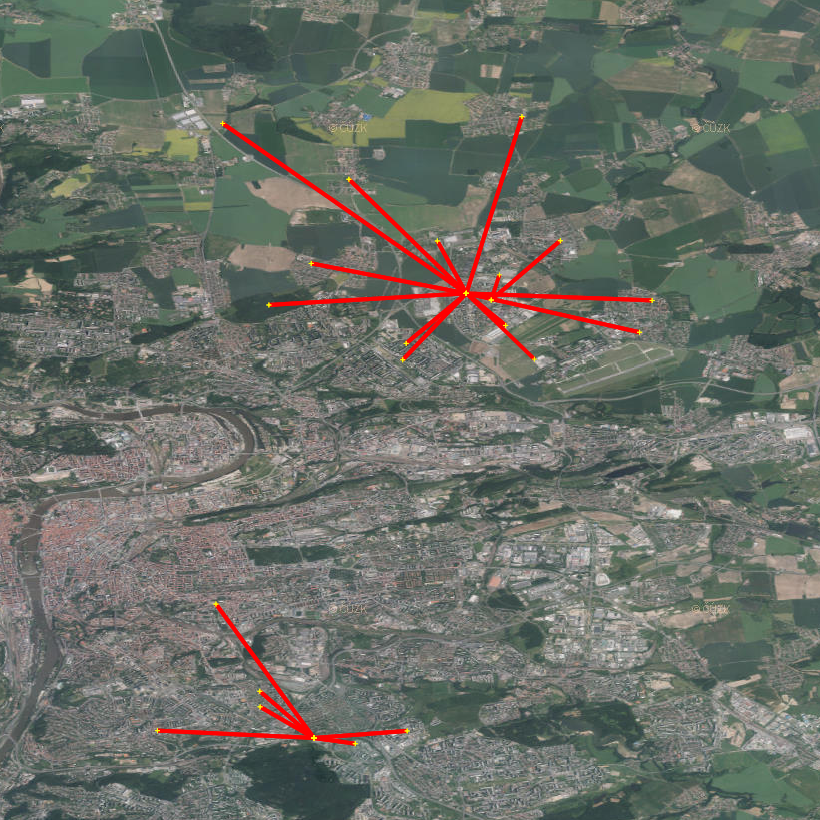
\includegraphics[width=0.5\textwidth]{./img/letnany.png}
    \caption[Snapshot model]{Současný stav k projektu dostupných MV spojů v Praze  \centering  }
        \label{fig:snapshot}
 \end{figure} 
Časový krok sběru dat není konstantní. Jednotlivé hodnoty jsou zaznamenávány do databáze časově nahodile. To je způsobeno přenosovými rychlostmi výpočetní techniky.  Referenční věž zaznamenává hodnoty v řádech sekund a ty jsou následně ukládány do databáze. Prakticky jsou data ukládána pro jednotlivé MV spoje přibližně po 15 sekundách. 


%\noindent \hrulefill % just for visual guide

\subsubsection{Databáze}  
Využitá databáze pro záznam dat z MV spojů je PostgreSQL, která data pro zmíněné lokality nepřetržitě od dubna 2013 ukládá. Dostupná data pro potřeby vývoje GIS modulu jsou v formě zálohy databáze (\textit{database dump}) časového rozsahu jednoho týdne sběru. Databáze obsahuje tabulky \texttt{link}, \texttt{node} a \texttt{record} 
\begin{table}[h]
\centering
\begin{tabular}{|lll|}
\hline
\multicolumn{1}{|c}{jméno tabulky} & \multicolumn{1}{c}{atributy}                                                    & \multicolumn{1}{c|}{popis} \\ \hline\hline
link   & \begin{tabular}[c]{@{}l@{}}linkid, rxoid, txoid\\ fromnode, tonode\end{tabular}    & definice spojů z vysílačů \\\hline
node   & \begin{tabular}[c]{@{}l@{}}ipaddres, lat, long \\ name, nodeid\end{tabular}        & geometrie vysílačů       \\\hline
record & \begin{tabular}[c]{@{}l@{}}linkid, time, frequency\\ rxpower, txpower\end{tabular} & naměřené hodnoty          \\ \hline
\end{tabular}
\caption{Přehled tabulek z databáze}
\label{tab:database}
\end{table}


\paragraph*{Tabulka link} obsahuje informace, ze kterých vysílačů (\texttt{fromnodeid, tonodeid}) jsou jednotlivé spoje \texttt{linkid} definovány. Ostatní atributy nebyli využity.


\begin{figure}[h!]
\centering
\footnotesize
\begin{BVerbatim}
 linkid |  ifname  |   rxoid    |   txoid    | fromnodeid | tonodeid 
--------+----------+------------+------------+------------+----------
     43 | 1/2.1/1  | 2129920257 | 2146697473 |         23 |       29
     44 | 1/16.1/1 | 2129922049 | 2146699265 |         29 |       23
     45 | 1/2.1/1  | 2129920257 | 2146697473 |         24 |       29
     46 | 1/6.1/1  | 2129920769 | 2146697985 |         29 |       24
\end{BVerbatim}
\caption{ Výpis dat s tabulky  \texttt{link} (limit 4) }
\end{figure}


\paragraph*{Tabulka node} obsahuje klíčové informace o poloze vysílačů v souřadnicovém systému WGS-84 (\texttt{lat, lon}).

\begin{figure}[h!]
\centering
\footnotesize
\begin{BVerbatim}
   ipaddress   |   lat   |  long   |  name  | nodeid 
---------------+---------+---------+--------+--------
 10.230.79.65  |  50.069 | 14.4534 | 10283A |     23
 10.230.79.93  | 50.0375 | 14.4848 | 10333A |     24
 10.230.80.245 | 50.0404 | 14.4965 | 12209A |     25
 10.230.79.69  | 50.0458 | 14.4633 | 12276A |     26
\end{BVerbatim}
\caption{Výpis dat s tabulky  \texttt{node} (limit 4)}
\end{figure}

\paragraph*{Tabulka record} má atributy time datového typu \texttt{timestamp}, dále \texttt{rxpower} a \texttt{txpower} jsou údaje o přijatém a odeslaném 

\begin{figure}[h!]
\centering
\footnotesize
\begin{BVerbatim}
 linkid |          time           | rxpower | txpower 
--------+-------------------------+---------+---------
     43 | 2013-09-08 23:59:14.913 |   -48.5 |      -3
     45 | 2013-09-08 23:59:15.334 |   -48.5 |      -4
     47 | 2013-09-08 23:59:15.755 |   -48.9 |       2
     49 | 2013-09-08 23:59:16.161 |   -48.9 |      -7
\end{BVerbatim}
\caption{Výpis dat s tabulky \texttt{record} (limit 4) }
\end{figure}


\subsubsection*{Úprava databáze}
\label{subsubsec:upravadatabaze}  
 V databázové dávce chybí atribut s informací o vertikální či horizontální polarizace signálu \texttt{polarization}, proto byl do tabulky \texttt{link} přidán ručně a následně i známé hodnoto pro jednotlivé spoje. V současné době probíhá jednání se správcem databáze v T-Mobile o přidání tohoto atributu.
 
Úprava databáze se provádí z prostředí modulu a je charakteristická následujícím postupem:
\begin{enumerate}
\item \textbf{Geometrie}- extenze PostGIS
\item \textbf{Indexy}- vytvoření indexů pro optimalizaci vyhledáván dotazů
\item \textbf{Funkce}- přidání agregačních funkcí pro statistické výpočty
\item \textbf{Konfigurace}- dílčí úpravy databáze pro výpočty
\end{enumerate}

\paragraph*{Geometrie} Do databáze byla přidána extenze PostGIS (\texttt{CREATE EXTENSION postgis}), která umožnila vytvořit geometrický atribut (geom) u tabulky node a link. Souřadnicový systém byl definován pro WGS-84 (SRID 4326).

Definování geometrického atributu (geom) datového typu POINT pro vysílače. 

\begin{footnotesize}
\begin{lstlisting}[style=mybash]
SELECT AddGeometryColumn ('public','node','geom',4326,'POINT',2)
\end{lstlisting}
\end{footnotesize}

Vytvoření geometrického atributu (geom) datového typu LINESTRING pro spoje. 

\begin{footnotesize}
\begin{lstlisting}[style=mybash]
SELECT AddGeometryColumn('public','link','geom',4326,'LINESTRING',2)
\end{lstlisting}
\end{footnotesize}

Definování geometrického atributu (geom) datového typu POINT. 

\begin{footnotesize}
\begin{lstlisting}[style=mybash]
UPDATE node SET geom = ST_SetSRID(ST_MakePoint(long, lat), 4326)
\end{lstlisting}
\end{footnotesize}

Pomocí funkce \texttt{ST\_MakeLine} byla rekonstruována geometrie spojů (\texttt{link}) z vysílačů (\texttt{node}). Z geometrie spojů (\texttt{link}) byla vypočtena jejich délka \texttt{ST\_Length}.

\paragraph*{Indexy} byly vytvořeny v tabulce \texttt{record} nad atributy time a recordid, pro následné výpočty s dotazováním databáze. K vytvoření indexů bylo využito algoritmu B-tree \footnote{\url{http://www.postgresql.org/docs/9.2/static/indexes-types.html}}

\begin{footnotesize}
\begin{lstlisting}[style=mybash]
--index b-tree pro atribut recordid
CREATE INDEX idindex ON record USING btree(recordid);		
\end{lstlisting}
\end{footnotesize}

\paragraph*{Funkce} je napsána v nativním jazyku PL/pgSQL a slouží pro výpočet statistické funkce modus pro zvolený atributový sloupec. 

\paragraph*{Konfigurace tabulek} databáze spočívá především v doplnění atributů vytvořením sekvencí a vymazáním záznamů rxpower=-99.9, které charakterizují výpadek spoje. 

\bigskip

Veškeré úpravy databáze se provádí automaticky pomocí modulu \textit{r.mwprecip} a jsou provedeny jen při prvním spuštění. 
\section{GRASS GIS modul}
Jedním z hlavních výsledků této práce je navržení a implementace modulu \textit{r.mwprecip} pro zpracování hrubých dat z MV spojů v GIS. K tomuto účelu byl zvolen systém GRASS GIS s využitím rozhraní \textit{GRASS Python Scripting Library}. V rámci vývoje byly vytvořeny dva moduly.

\paragraph*{r.mwprecip}  modul, který tvoří hlavní GIS nástroj pro zpracování dat z externí databáze.
\paragraph*{v.link.precip} je sekundárním  k modulu  \textit{r.mwprecip}, jehož funkcionalita spočívá v nativním přístupu k výsledkům   v GRASS GIS.  

\subsubsection{Použité knihovny}
Při psaní programu bylo využito jazyku Python, který je podporován knihovnou  \textit{GRASS Python Scripting Library}\cite{spygrass}. Ta umožňuje zjednodušené volání GRASS modulů. Mimo to bylo využito dílčích částí standardní knihovny \textit{The Python Standard Library}\footnote{\url{https://docs.python.org/3.4/library/}} verze 3.4

Knihovna psycopg\footnote{\url{http://initd.org/psycopg/docs/}} je v jazyce Python a  umožňuje přístup z klientské strany do databáze PostgreSQL. Této knihovny bylo využito pro veškerý přístup do databáze, mimo přístupu z GRASS modulů s využitím \textit{GRASS Python Scripting Library}.

\subsubsection{Uživatelské rozhraní}
Uživatelské rozhraní částečně vyplývá z možností \textit{GRASS Python Scripting Library}, kde při tvorbě modulu jsou jednotlivé ovládací prvky v podobě přepínačů a parametrů.\ref{subsubsec:grassterminologie}. Program se ovládá (spouští) bud s příkazové řádky GRASS nebo ve wxGUI, kde se vygeneruje programové okno s jednotlivými sekcemi programu. 

\begin{figure}[h!]
    \centering
    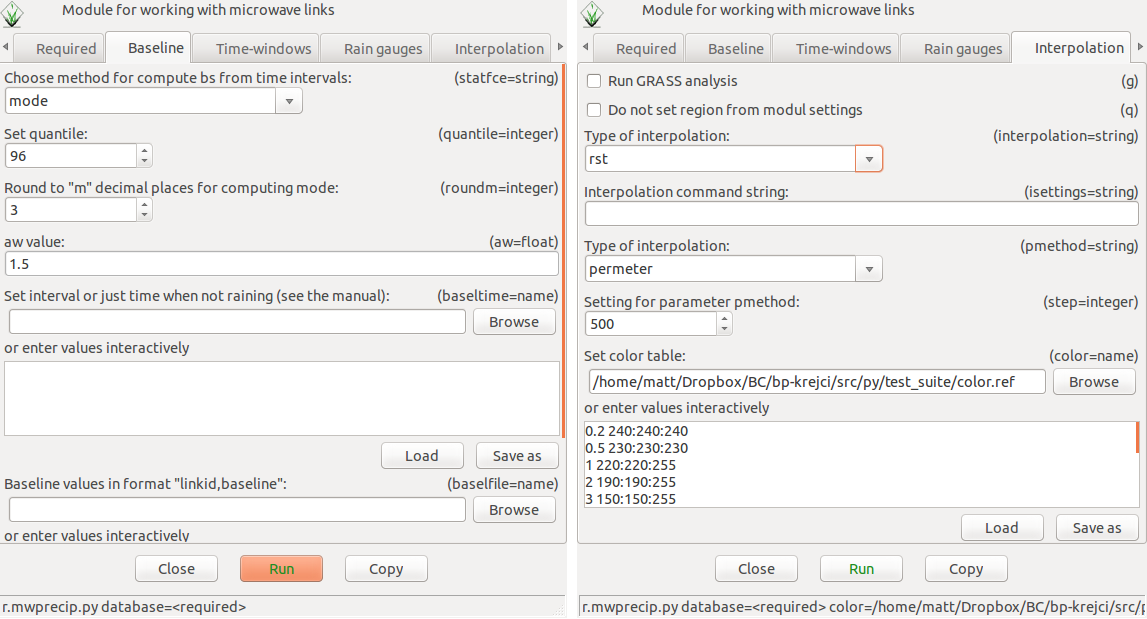
\includegraphics[width=\textwidth]{./img/grass/gui.png}
    \caption[GUI modul]{Ukázka GUI r.mwprecip sekce Baseline a Interpolation  \centering  }
        \label{fig:baseline}
 \end{figure}

\subsection{Modul r.mwprecip}
Primární účel  modulu \textit{r.mwprecip} je zpracování hrubých dat do takové formy, která je rozhraní GRASS GIS vlastní. Základní funkčnost modulu spočívá jak ve zpracování dat, tak ve výstupu vhodném pro GIS analýzy. Modul pro výstupní data podporuje dvě základní geodatové reprezentace. Výstupem jsou jak interpolované srážky v rastrové podobě, tak vektorová reprezentace pro jednotlivé MV spoje. 
Zpracování dlouhých časových řad po zvoleném intervalu je výhodné pro časoprostorové analýzy, pro které je nově v \textit{GRASS GIS 7} implementován \textit{Temporal GRASS GIS framework}.





 
\subsubsection{Funkcionalita a ovládání}
V následujícím textu jsou shrnuty vlastnosti modulu \textit{r.mwprecip}. Funkcionalita modulu \textit{r.mwprecip} se dělí do tří dílčích částí.
\begin{itemize}
\item Výpočet srážek
\item Vytvoření časových oken
\item Plošné interpolace 
\end{itemize}

Jediným povinným parametrem (\textit{Required}) modulu \textit{r.mwprecip} je \texttt{database}, jehož vstupem je textový řetězec v s názvem databáze PostgeSQL. Modul je koncipován pro experimentální účely, kde se předpokládá práce na lokálním počítači bez přihlašovacího jména a hesla k databázi. V opačné případě je možnost v poslední sekci \textit{Database} definovat vstupní hodnoty pro parametry \texttt{user} a \texttt{password}


\begin{table}[h]
\centering
\begin{tabular}{|lll|}
\hline
\multicolumn{1}{|c}{sekce} & \multicolumn{1}{c}{parametry/ přepínače}                                                    & \multicolumn{1}{c|}{popis}    \\ \hline\hline
Required                   & database                                                                                    & jméno databáze s daty         \\\hline
Baseline                   & \begin{tabular}[c]{@{}l@{}}statfce quantile roundm\\aw baseltime baselfile\end{tabular}    & nastavení výpočtu baseline   \\\hline
Time-windows               & \begin{tabular}[c]{@{}l@{}}interval fromtime\\totime lignore\end{tabular}                 & nastavení časových oken       \\\hline
Rain Gauges                & rgauges                                                                                     & nastavení vstupu srážkoměrů   \\\hline
Interpolation              & \begin{tabular}[c]{@{}l@{}}-g -q interpolation isettings\\pmetohod step color\end{tabular} & nastavení interpolací a barev \\\hline
Database                   & user password                                                                               & doplňkové nastavení db        \\\hline
Optional                   & -p -r schema                                                                                & informace o db, smazání temp, \\ \hline
\end{tabular}

\caption{Přehled parametrů v jednotlivých GUI sekcích}
\label{tab:rozhrani}
\end{table}


Při každém uživatelském spuštění modulu \textit{r.mwprecip } proběhne kontrola stavu databáze. Při prvním spuštění je databáze uvedena do potřebného stavu \ref{subsubsec:upravadatabaze}. Filosofie modulu je založená na předpokladu, že bude sloužit k experimentálním pokusům v rozhraní GRASS GIS. Jednotlivé kroky výpočtů jsou od sebe separovány, aby se při změně parametrů jen části programu se nemusely provádět veškeré výpočty znovu. Dělí se do výše zmíněných tří kategorií. 

Modul pracuje v oddělených databázových schematech. Ze schéma \texttt{public} načítá veškerá data z databáze a až na prvotní jednorázovou úpravu databáze do ně nezapisuje. Výsledky dílčích tří kategorii jsou zapisovány do pracovního schématu, který si uživatel pojmenuje pomocí parametru \texttt{schema}. Pomocí volby různých názvů je možné vytvářet schémata pro dané konfigurace výpočtu a zpětně se k nim vracet.

Modul zapisuje konfiguraci nastavených výpočtu do textových souborů, které jsou uloženy ve složce s názvem zvoleným pro pracovní schéma (parametr \texttt{schema}). Složka je umístěna ve spouštěcím adresáři modulu. Při dalším spuštění modul porovnává nastavení s konfiguračními soubory a na základě toho provede jen konfiguračně pozměněnou část výpočtu. 

V sekci \textit{Optional} je přepínač \texttt{-r}, který odstraní uživatelské schéma a složku s konfiguračními soubory. Této funkce se může využít pro vrácení databáze do původního stavu, nebo například při nekorektním ukončení modulu či výpočtu.


\paragraph*{Výpočet srážek} je při opominutí přípravy databáze první částí, která vychází z \acs{GUI} sekce \textit{Baseline}. Při konfiguraci volby výpočtu baseline se vypočtené srážky zapíší do pracovního schématu, které se vytvoří v databázi.

Baseline jde určit jak ručně a tak i výpočtem z období kdy neprší. 
Pro ruční zadání hodnot slouží parametr \texttt{baselfile}, do kterého jsou vstupními hodnotami id. spoje (\texttt{linkid}) a hodnota o baseline (typ real) ve formátu \acs{CSV}.
\begin{table}[h!]
\centering
\begin{tabular}{|lll|}
\hline
\multicolumn{1}{|c}{parametr} & \multicolumn{1}{c}{typ} & \multicolumn{1}{c|}{explicitní hodnoty}                                \\ \hline\hline
statfce                                & string                  & \begin{tabular}[c]{@{}c@{}}mode avg quantile\end{tabular}     \\
quantile                               & integer                 & 1-100                                                         \\
roundm                                 & integer                 & -                                                             \\
aw                                     & float                   & -                                                             \\
baseltime                              & soubor         		 & interaktivní zadání                                           \\
baselfile                              & soubor         		 & interaktivní zadání                                           \\ \hline
\end{tabular}
\caption{Parametry v GUI sekci Baseline}
\label{my-label}
\end{table}
Druhou možností je poloautomatizovaný výpočet, kdy jsou vstupními údaji časové intervaly, nebo okamžiky, které představují suché období. První řádek označuje časový okamžik suchého období, na dalším řádku je časový interval  uvozeny řetězcem \texttt{int} a za ním nasledují dva řádky definující interval. Další řádek reprezentuje jeden zvolený časový okamžik. 


\begin{figure}[h!]
\begin{footnotesize}
\lstset{extendedchars=false,
escapeinside=''}
\begin{lstlisting}[style=mybash]
2013-09-09 07:00:00     -'č'asov'ý' okam'ž''i'k	
int                     -uvozen'í' intervalu
2013-09-10 04:00:00     -za'č''á'tek obdob'í'
2013-09-10 05:00:00     -konec obdob'í'
2013-09-13 04:55:00     -'č'asov'ý' okam'ž''i'k	
\end{lstlisting}
\end{footnotesize}
\end{figure}


Po zvolení suchých období je možnost volby výpočtu výsledné baseline pro daný spoj pomocí základních statistických funkcí. K volbě slouží parametr \texttt{statfce}, která má explicitně nastavené možnosti \emph{avg} (průměr), \emph{mode} (modus), \emph{quantile} (kvantil). Výchozí hodnota je nastavena na mode. Při volbě funkce modus je možné nastavit počet desetinných míst při zaokrouhlení vzorku hodnot. Parametr \texttt{quantile}  vyjadřuje horní kvantil souboru dat v procentech. 

Posledním parametrem v této sekci je \texttt{aw} a vyplývá ze vztahu \ref{eq:Ar}.


\paragraph*{Časová okna} jsou druhou samostatnou GUI sekcí s názvem \textit{Time-windows}. Vytvoření časových oken přímo navazuje na vypočtené hodnoty. Principiálně jde o vytvoření tabulek vždy pro jeden časový okamžik. K tomu je třeba z náhodného časového kroku vytvořit krok konstantní.

K volbě časového intervalu po kterém chceme okna vytvářet slouží parametr \texttt{interval}, který je explicitně nastaven na hodnoty \emph{minute} (minuta), \emph{hour} (hodina) a \emph{day} (den). Minuta je nastavena jako výchozí.  Například při volbě \emph{minute} jsou spočtené srážky cca po 15 [s] zprůměrovány a výsledná hodnota je za minutu . Průměrná hodnota je vždy uváděna v intenzitě srážek v [$mm \cdot h^{-1}$], i v případě vytváření časových oken po dni či minutě.
\begin{table}[h]
\centering
\begin{tabular}{|lll|}
\hline
\multicolumn{1}{|c}{parametr} & \multicolumn{1}{c}{typ} & \multicolumn{1}{c|}{explicitní hodnoty} \\ \hline\hline
interval                               & string                  & minute, hour, day             \\
fromtime                               & timestamp               & YYYY-MM-DD H:M:S              \\
roundm                                 & integer                 & YYYY-MM-DD H:M:S              \\
lignore                                & soubor                  & linkid                        \\ \hline
\end{tabular}
\caption{Parametry v GUI sekci Time-window}
\label{my-label}
\end{table}
Oproti výpočtu srážek je vytvoření časových oken možno ohraničit intervalem, ze kterého mají být okna vytvořena. Tato volba má přímou návaznost na plošnou interpolaci srážek, či časoprostorové analýzy. Vstupní hodnoty pro parametry fromtime(začátek intervalu) a totime(konec intervalu) jsou časového datového typu (timestamp) ve formátu \emph{"YYYY-MM-DD H:M:S"}. V sekci \textit{Optional} je přepínač \texttt{-p} který vypisuje do informačního terminálu informaci o začátku a konci časového rozsahu datasetu.

Parametr \texttt{lignore} jehož vstupní hodnotou soubor, definuje jednotlivé spoje, které mají být z časových oken vynechány. tato funkce je vytvořena k zamezení přidání rozbitých, či divně se chovajících spojů do časových oken, které by tak ztrácela validitu. Hodnoty \texttt{linkid} se zadávají po jednom řádku vždy ve formátu datového typu (int) odvozeným z databázové tabulky \texttt{link}.

Další možností je načtení časových řad ze srážkoměrů pomocí parametru \texttt{rgauges}. Srážkoměrná data jsou načítána v předzpracovaném stavu a to v časových řadách s hodnotou intenzity srážky v [$mm \cdot h^{-1}$]. Formát vstupního souboru je následující.


\begin{figure}[h!]
\begin{footnotesize}
\lstset{extendedchars=false,
escapeinside=''}
\begin{lstlisting}[style=mybash]
2                             #id sr'á''ž'kom'ě'ru			
50.151634                     #WGS84 'š''í''ř'ka				
14.508727                     #WGS84 d'é'lka	
2013-09-01 00:00:00,6.12      #hodnoty ve form'á'tu CSV 
2013-09-01 00:01:00,12.18     #"YYYY-MM-DD H:M:S,hodnota"		
2013-09-01 00:02:00,12.12

\end{lstlisting}
\end{footnotesize}
\end{figure}


Vstupem do parametru \texttt{rgauges} je cílová složka se soubory, které jsou načteny dávkově. Jednotlivým srážkoměrům se vytvoří vektorová geometrie reprezentovaná body a ta se uloží do databáze PostgreSQL. Pro vytvoření časových oken z dat srážkoměrů slouží z podstaty věci stejné nastavení pr tvorbu časových oken jako pro intenzity srážek z MV spojů.


\paragraph*{Interpolace} je jedním z výstupů modulu \textit{r.mwprecip}. GUI sekce \textit{Interpolation} je specifická dvěma částmi. První zahrnuje interpolace bodů podél spojů a druhá plošné interpolace srážek.

Nastavení  výpočetního regionu je možné pomocí přednastavených hodnot modulu \textit{r.mwprecip}. Při uživatelské volbě z GRASS modulu g.region je možné tuto automatizaci vypnout přepínačem \texttt{-q}
\begin{table}[h]
\centering
\begin{tabular}{|lll|}
\hline
\multicolumn{1}{|c}{parametr} & \multicolumn{1}{c}{typ} & \multicolumn{1}{c|}{explicitní hodnoty} \\ \hline\hline
interpolation                          & string                  & rest, idw, bspline           \\
isettings                              & string                  &                              \\
pmethod                                & integerstring           & permeter, count              \\
step                                   & integer                 &                              \\
color                                  & string                  & hodnota R:G:B                \\ \hline
\end{tabular}
\caption{Parametry v GUI sekci Interpolation}
\end{table}
Současná verze GRASS GIS neumožňuje interpolace z liniové reprezentace dat, což není nijak neobvyklé při porovnání s ostatními nástroji GIS. Parametr \texttt{pmethod} definuje metodu interpolace bodů podél spojů. Explicitně je nastaven na hodnotu \emph{permeter} (po metrech) a při volbě této metody je provedena interpolace bodů v pevně stanoveném kroku po metrech [m], který vychází z parametru \texttt{step}. Parametr \texttt{step} je využit i k definování hodnoty k druhé explicitní hodnoty \emph{count} (číslo). Hodnota \emph{count} rozloží rovnoměrně podél MV spojů daný počet bodů (\texttt{step}).

Plošné interpolace využívají dostupných modulů v GRASS. Interpolace je možné definovat jak uživatelsky tak automaticky (výchozí hodnoty jednotlivých modulů). Pro volbu interpolace s výchozími hodnoty slouží parametr \texttt{interpolation}, který je explicitně nastaven na \emph{rst}(regular spline tension), \emph{idw} (invese distace weighting) a \emph{bspline} (bicubic spline tension). 

Druhou možností je uživatelského nastavení jednotlivých interpolací. Pro ty slouží parametr \texttt{isettings}, do kterých je vstupem textový řetězec definovaný ve formátu \textit{GRASS Python Scripting Library}. Je možné tyto řetězce nakonfigurovat pomocí wxGUI a z výstupního terminálu zkopírovat. Řetězec s parametry a přepínači musí být uvozen do závorek ve formátu:     

\begin{figure}[h!]
\begin{footnotesize}
\lstset{extendedchars=false,
escapeinside=''}
\begin{lstlisting}[style=mybash]
grass.run_command()                                                           
\end{lstlisting}
\end{footnotesize}
\end{figure}
Jednotlivé parametry v řetězci musí být odděleny čárkou ",".

Některé parametry (vstupní/výstup mapa) pro dané interpolační metody musí být nastaveny pro správné fungování dle tabulky\ref{tab:interpol}.


\begin{table}[h]
\centering
\begin{tabular}{|lll|}
\hline
\multicolumn{1}{|c}{interpolace} & \multicolumn{1}{c}{parametr} & \multicolumn{1}{c|}{hodnota} \\ \hline\hline
\multirow{3}{*}{r.surf.rst}      & input                        & points\_nat                  \\
                                 & elevation                    & out                          \\
                                 & zcolumn                      & attribute\_col               \\\hline
\multirow{3}{*}{r.surf.idw}      & input                        & points\_nat                  \\
                                 & output                       & out                          \\
                                 & column                       & attribute\_col               \\\hline
\multirow{3}{*}{r.surf.bspline}  & input                        & points\_nat                  \\
                                 & raster\_output               & out                          \\
                                 & column                       & points\_nat                  \\ \hline
\end{tabular}
\caption{Povinné nastavení parametrů pro jednotlivé interpolační moduly.}
\label{tab:interpol}
\end{table}



Příkladem může být interpolace IDW (r.surf.idw) s parametry pro nastavení hodnoty exponentu \texttt{power} a počtu bodů \texttt{npoints} ze které se daná buňka interpoluje. 

\begin{figure}[h!]
\begin{footnotesize}
\lstset{extendedchars=false,
escapeinside=''}
\begin{lstlisting}[style=mybash]
#Uk'á'zka mo'ž'n'é'ho vstupu parametru isettings
grass.run_command( "v.surf.idw", input=points_nat,
column=attribute_col, output=out, npoints=25, power=2.5 )                            
\end{lstlisting}
\end{footnotesize} 
\end{figure}


 
\subsubsection{Vstup a výstup modulu}
\paragraph*{Vstup} hlavní datový vstup do modulu představuje konektivita s externí databází PostgreSQL. V ní byl uložen zmíněný vzorek dat.
Modul dále podporuje dávkové načítání časových řad ze srážkoměru.
\paragraph*{Výstup}
Jedním z možných výstupů jsou vypočtené srážkové intenzity uložené v \textbf{databázi}. Ty jsou uloženy jak v časovém kroku sběru dat, tak ve zvoleném kroku. Pro zvolený časový krok se vytvářejí tabulky představující jednotlivá "časová okna", která jsou vhodná pro následné analýzy v GIS.
\textbf{Rastrová data}  reprezentují výsledek zvolené plošné interpolace vypočtených srážek.
\textbf{Vektorová data} jsou vytvořena na základě polohových údajů o telekomunikačních spojích v databázi a jsou reprezentována  liniemi a  interpolovanými body podél MV spojů, ke kterým jsou pomocí modulu v.link.precip připojována jednotlivá časová okna z databáze.



\subsection{Modul v.link.precip}
Hlavní funkcionalita modulu spočívá ve zjednodušeném přístupu k výsledkům z primárního modulu. Modul \textit{r.mwprecip} při vytváření časových oken zapisuje tabulky do databáze. Vektorová geometrie reprezentovaná liniemi (MV spoje) a body (interpolace)  je v databázi pro zamezení redundance dat v samostatné tabulce, nikoliv pro každé časové okno. Pro analýzy a další využití výsledků v GRASS GIS, je podstatné, aby bylo možné jednotlivá časová okna připojovat k vektorovému podkladu a s vhodnou tabulkou barev je zobrazovat. 
Toho lze docílit sledem po sobě jdoucích volání jednotlivých modulů v GRASS. Pro jednoduchost byl vytvořen  modul \textit{v.link.precip}, který to umožňuje v uživatelsky přístupně formě. 


\subsubsection{Funkcionalita a ovládání}
Modul při prvním spuštění vytvoří vektorovou vrstvu v nativním prostředí GRASS na základě vytvořené geometrie v databázi PostgreSQL. Dále pak připojí nastavenou tabulku reprezentující časové okno. Při dalším připojení jiného časového okna je bývalá připojená tabulka odpojena a k té samé vektorové vrstvě se připojí nová. Modul je tvořen dvěma GUI záložkami \textit{Required} a \textit{Optional}. 

První záložka \textit{Required} obsahuje jen povinné parametry.  Parametr \texttt{schema}  označuje pracovní schéma, ve kterém jsou uloženy výsledky pro  zobrazení. Druhým parametrem je časová známka (timestamp) časového okna, které chceme připojit k vektorovému podkladu(spoje). Výsledná vektorová mapa je vždy pojmenována \textit{"link\_nat"}. Další parametr  \texttt{type} je  explicitně nastaven na hodnoty \emph{links} a \emph{raingauge}. Při využití načítání srážkoměrných dat v modulu r.wmprecip, je možné připojit k bodové vrstvě "gauge\_nat" tabulku s časovým oknem stejně jako v případě výsledku pro MV spoje.

Druhá záložka \textit{Optional} obsahuje  tři přepínače a jeden parametr.  Přepínače jsou definovány:
\begin{description}
\item[-c]   slouží pro případ, kdy bude nutno pracovat s více časovými okny najednou. Přepínač \texttt{-c} časová okna nepřipojuje k vektorové vrstvě \textit{"link\_nat"}, ale vytváří nové s názvem ("view" + <hodnota timestamp>). Při této volbě dochází k redundanci dat vektorových vrstev.
\item[-p] vypíše do výstupové řádky hodnoty připojené atributové tabulky.
\item[-r] smaže dočasné  soubory z pracovního schéma.
\end{description}

Tabulka barev pro vektorovou vrstvu je možná nastavit parametrem \texttt{color}, jehož vstupní hodnota je textový soubor  analogický k formátu tabulky barev pro plošné interpolace.

\section{Výstupy modulu a využití}

V následujících ukázkách plošných map z jednotlivých interpolací bylo využito vektorových vrstev linií a bodů ke znázornění realně spočtené srážky z MV spojů. Vektorové linie znázorňují spoje. Čtverce vyjadřují body, ze kterých se spočetla interpoalce. Barva čtverce vyjadřuje intenzitu srážek stejné tabulky barev. 


\subsection{Vizualizace}
Zobrazení srážkových intenzit byl jedním z nároku na funkčnost GIS aplikace. Primárně pro umožnění lepšího a rychlejšího vhledu do a pro lepší orientaci při rozborech naměřených dat.

Vizualizovat je možné plošná srážková data, která jsou odhadem interpolačních metod. K vizualizaci je vytvořena tabulka barev odvozena od standardní  stupnic pro srážková data. Druhou možností je vizualizace liniová a bodová připojením jednotlivých časových oken k vektorové vrstvě (v.link.precip). Modul \textit{v.color} umožňuje definovat barvu vektorové vrstvy na základě přiřazené tabulky barev pro atributový sloupec v databázi.

Modul \textit{g.gui.animation} je interaktivní a uživatelsky přístupný wxGUI modul, který umožňuje vytvářet animace z jednotlivých po sobě jdoucích časových oken. Těžiště jeho výhod bude při vizualizaci srážkových map v čase. 

\subsubsection{Plošná interpretace srážek}
Výsledek plošných interpolací  je ovlivněn mnoha faktory, které se podílejí na správnosti interpolovaných  hodnot. Obecně interpolace z liniových vektorů je v GIS neobvyklá a jediným východiskem pro využití podporovaných interpolačních metod v GRASS je nahrazení liniové reprezentace body. 

Tento postup poukazuje na zcela novou problematiku interpolačních metod. MV spoje jsou poměrně hustě rozloženy a z toho plyne  velká variabilita v rozložení a volbě počtu bodů. Optimální rozložení bodů je patrně také závislé na zvolené interpolační metodě.

Dalším charakterem ne zcela typickým je hustota MV sítě dostupného vzorku. Skládá se ze dvou referenčních vysílačů, které jsou od sebe s porovnáním s reálnou  hustotou vysílačů velmi vzdálené. Při využití disponibilních vysílačů např. v sítí T-mobile, by prostorovou mezeru doplnilo několik desítek až stovek dalších. Tím jsou výstupy následujících interpolací oproti možným výsledkům zkresleny. Možným východiskem  problému nízké hustoty vzorku je zvolit výpočetní region jen pro jeden referenční vysílač. Této úvaze ale odporuje charakteristika topologie spojů, které jsou prostorově rozloženy do tvaru hvězdic a v mnoha případech by se jednalo o extrapolaci budu.

V následujících ukázkách plošných interpolací jsou představeny použitelné  metody pro datový výstup z vytvořeného modulu.

\paragraph*{Rozlišení a region} bylo nastaveno pomocí výchozí hodnoty modulu \textit{r.mwprecip}, tedy:
\begin{figure}[h!]
\begin{footnotesize}
\lstset{extendedchars=false,
escapeinside=''}
\begin{lstlisting}[style=mybash]
        grass.run_command('g.region',
                          vect='link',
                          res='00:00:01',
                          n='n+ 00:00:20',
                          w='w-00:00:20',
                          e='e+00:00:20',
                          s='s-00:00:20')
\end{lstlisting}
\end{footnotesize} 
\end{figure}



\subsubsection*{v.surf.bspline}
Modulu \textit{v.surf.bspline} má parametr \texttt{method}, který umožňuje volby bilineární a bikubické interpolace.

\begin{description}
\item Parametry \texttt{sie} a \texttt{sin}, určují vzdálenost spline křivky pro jednotlivé kroky ve směrech východ-západ (sie) a sever-jih (sin). Maximální hodnota pro oba směry je 150 \texttt{sie}. 
<<<<<<< HEAD
\item Parametr \texttt{lambda\_i} (Thykonov regularization parameter) ovlivňuje vyhlazení interpolace. Při volbě malé \texttt{lambda\_i} jsou interpolované hodnoty více závislé na vstupních hodnotách; vysoké \texttt{lambda\_i} vytvoří výsledný rastr více jemný. Pro optimální zjištění parametru slouží přepínač \texttt{-c}, který pro nastavenou délku křivky spline vypočte RMS charakteristiky.
=======
\item Parametr \texttt{lambda\_i} (Thykonov regularization parameter) ovlivňuje vyhlazení interpolace. Při volbě malé \texttt{lambda\_i} jsou interpolováné hodnoty více závislé na vstupních hodnotách;vysoké \texttt{lambda\_i} vytvoří výsledný povrch více jemný. Pro optimální zjištění parametru slouží přepínač \texttt{-c}, který pro nastavenou délku křivky spline vypočte 
>>>>>>> 486fc15b9d842cf622696ed3a3e0f8ed427fe784
\end{description}


Parametry byly zvoleny $sin=0.01, sie=0.01$ a následně přepínačem \texttt{-c} spočteny RMS pro dané nastavení pro různé \texttt{lambda\_i} 
\begin{figure}[h!]
\begin{footnotesize}
\lstset{extendedchars=false,
escapeinside=''}
\begin{lstlisting}[style=mybash]
Table of results:
v.surf.bspline complete. Cross validation finished \
sie = 0.010000 and sin = 0.010000
    lambda |       mean |        rms |
   0.00010 |    -1.7025 |     9.7532 |
   0.00100 |    -1.7106 |     9.6971 |
   0.00500 |    -1.6996 |     9.5957 |
   0.01000 |    -1.6824 |     9.5004 |
   0.02000 |    -0.6679 |     9.5563 |
   0.05000 |    -0.4219 |     9.8108 |
\end{lstlisting}
\end{footnotesize} 
\end{figure}


\begin{figure}[h!]%
    \centering
    \subfloat[Bikubická interpolace- 1 bod]{ 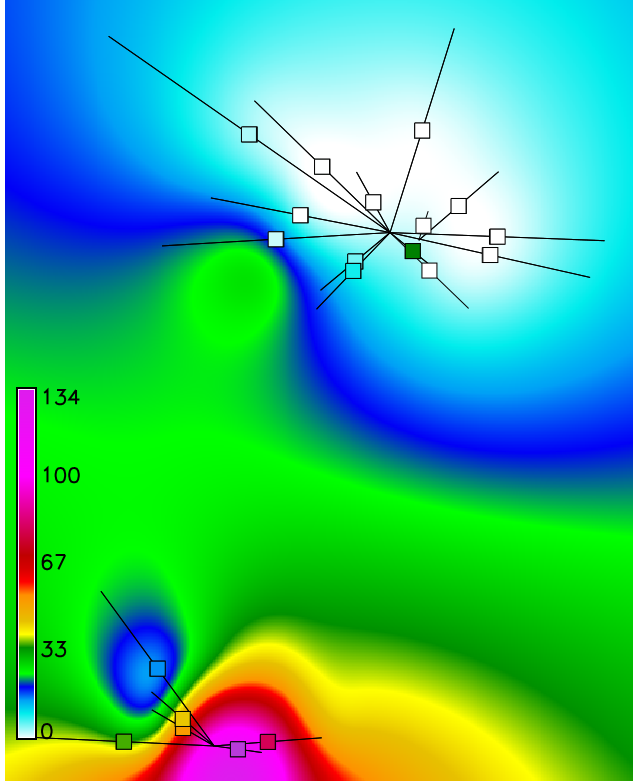
\includegraphics[width=0.3\textwidth]{./img/intanalys/bic1.png} }%
    \qquad
    \subfloat[Bikubická interpolace body po 500m]{ 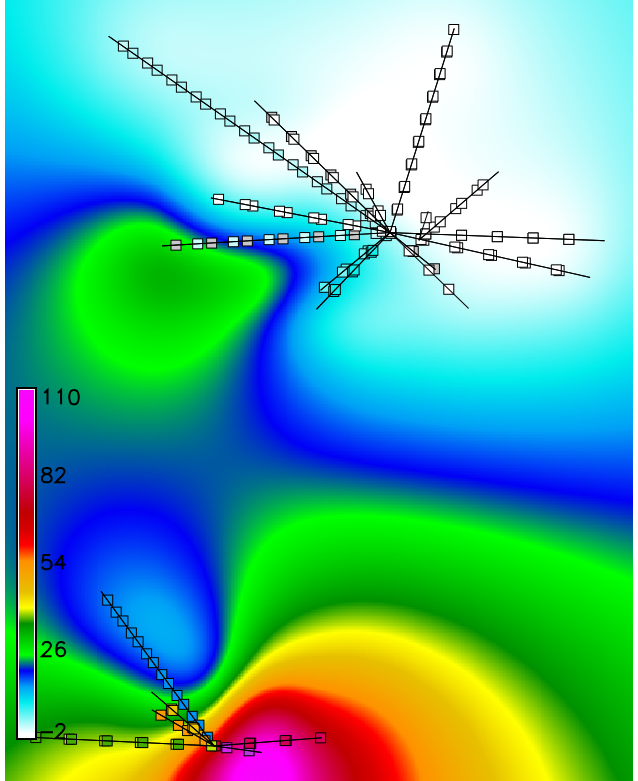
\includegraphics[width=0.3\textwidth]{./img/intanalys/bic500.png} }%
    \caption[Interpolace Bicubic]{Konfigurace parametrů a) sie=sin=0.01, lambda\_i=0.05; b) sie=sin=0.01, lambda\_i=0.01 \centering}%
    \label{fig:example}%
\end{figure}



\subsubsection*{v.surf.idw}
Modul \texttt{v.surf.idw} umožňuje nastavení exponentu \texttt{power} a počet známých bodů\texttt{npoints}, ze kterého se odhadovaný bod určuje\ref{sec:plostneinterpolace}. 

Metoda IDW v GRASS nedisponuje některými nastavením, které by bylo pro odhad plošných srážek pomocí MV vhodné. Jedním z nastavení je podpora rozdělení na sektory, která by byla v tomto případě výhodná pro rozdělení interpolované mapy na segmenty. Z daných segmentů by se do výpočtu neznámé buňky zahrnoval zvolený počet bodů. Dalším důležitým omezením u IDW je určení vzdálenostní bariéry, která ignoruje vzdálené body do výpočtu.

Z volby možných dvou parametrů vyplynulo několik poznatků

\begin{description}
\item Volba počtu bodů, ze kterých se provádí interpolace má velký vliv na možné výsledky. IDW je vhodná interpolační metoda pro rovnoměrně rozmístěné známé body. V tomto případě je vhodné výpočetní region rozdělit do dvou částí, čim se  do jisté míry nahradí chybějící parametr pro maximální vzdálenost. Rozdělení regionu se dá do jisté míry suplovat parametrem \texttt{npoints}, ale v případě dvou ohnisek bodů s rozdílnou hustotou, což koresponduje s topologii dostupného vzorku dat, tento úsudek neplatí. Výsledná mapa obsahuje na pomyslném spoji dvou regionů jednotlivých ohnisek bodů neplynulí přechod způsobený limitem \texttt{npoints}.
\item Volba exponentu ovlivňuje váhu (vzdálenost) jednotlivých bodu. Při volbě vysokého exponentu je odhadovaná buňka vypočtena s velikou váhou nejbližších známých bodu. S přímou návazností na volbu exponentu je  metoda IDW charakteristická tvořením interpolačních artefaktů v podobě koncentrických isolinií, které se často nazývají "\textit{bull eyes"}(býčí oči). 
\end{description} 

\begin{figure}[h!]%
    \centering
    \subfloat[IDW interpolace- 1 bod]{ 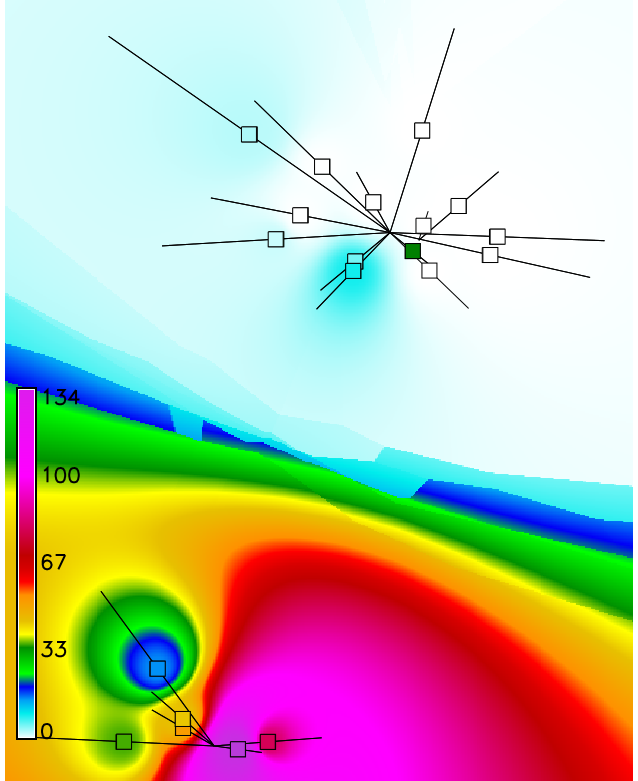
\includegraphics[width=0.3\textwidth]{./img/intanalys/idw1.png} }%
    \qquad
    \subfloat[IDW interpolace body po 500m]{ 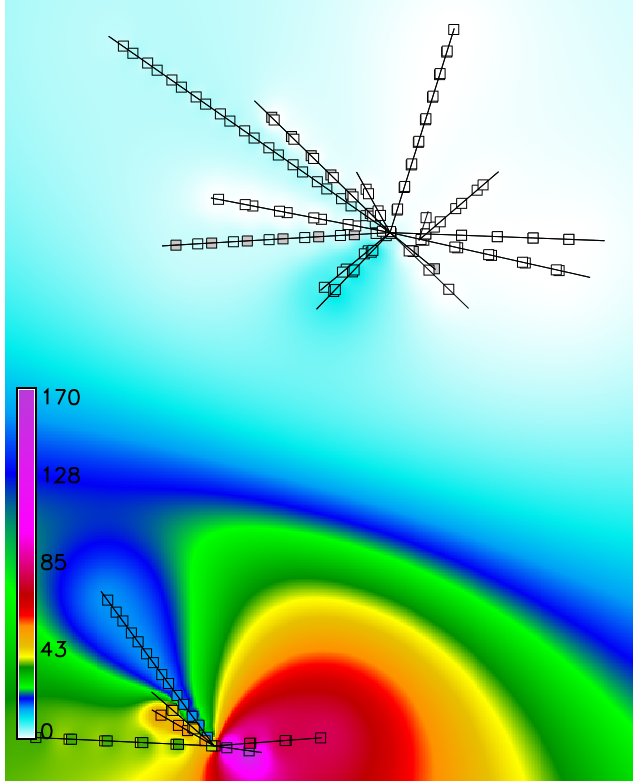
\includegraphics[width=0.3\textwidth]{./img/intanalys/idw500.png} }%
    \caption[Interpolace IDW]{Konfigurace parametrů IDW a) npoints=15, power=1.5; b) npoints=150, power=1.5\centering}%
    \label{fig:example}%
\end{figure}

Jednou z možných chyb interpolace IDW je přenesení hodnoty (srážek) přes mezilehlý známý bod. V praxi pak dochází k tomu, že vysoké srážkové intenzity ze známého bodu mohou přeskočit oblast  se známou nulovou srážkou a použít ji pro výpočet zcela špatně.



\subsubsection*{v.surf.rst}
Metodu RST představuje v GRASS modu \textit{v.surf.rst}, který je oproti modulu \textit{v.surf.idw} disponuje mnoha funkcemi a volbou parametrů.

\begin{description}
\item Parametry \texttt{dmin} a \texttt{dmax} umožňují nastavit minimální a maximální vzdálenost mezi body.
\item Parametr \texttt{tension} určuje napětí povrchu
\end{description}


\begin{figure}[h!]%
    \centering
    \subfloat[RST interpolace- 1 bod]{ 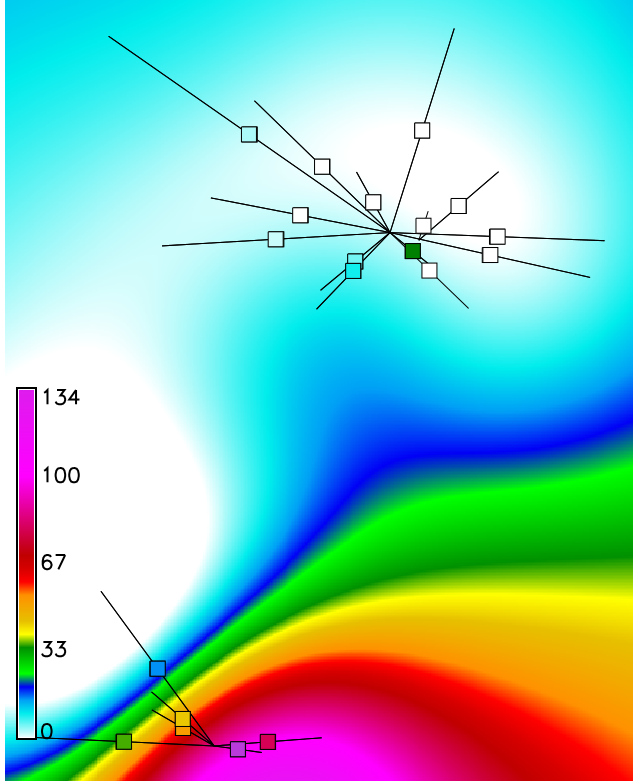
\includegraphics[width=0.3\textwidth]{./img/intanalys/rst1.png} }%
    \qquad
    \subfloat[RST interpolace body po 500m]{ 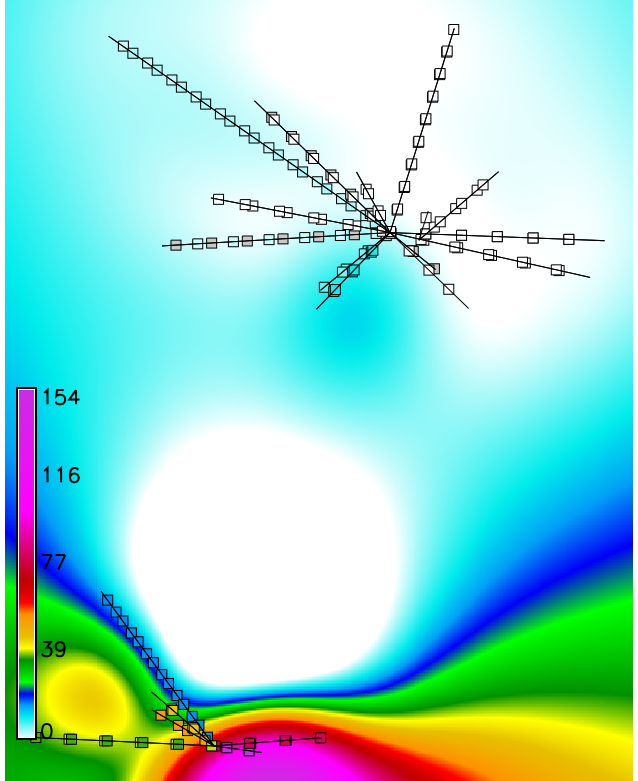
\includegraphics[width=0.3\textwidth]{./img/intanalys/rst500.png} }%
    \caption[Interpolace RST]{Konfigurace parametrů RST a)tension=30; b)tension=20 \centering}%
    \label{fig:example}%
\end{figure}


\paragraph*{Zhodnocení}  Výše byly uvedeny tři možné metody s různou konfigurací bodů a interpolačních parametrů. Už z vizualizací je patrné, že jednotlivé výsledky nabývají rozdílných hodnot a to jak napříč metodami, tak při rozložení bodů. Tento fakt je  ovlivněn rozložením bodu, které není svým rozsahem v dostupném datovém vzorku podloženo na reálné hustotě bodů pro tuto oblast. Výše uvedený krátký přehled plošných interpolací naznačuje možnosti nových směrů bádání v oblasti MV spojů ve spojení s plošnou reprezentací srážek. 


\subsection{Temporal GRASS framework}
Kapitola \textit{Temporal GRASS framework} poukazuje na možné využití \textit{Teporal GRASS framework (TGASS)}, který je nově ve verzi GRASS GIS 7. Hlavním cílem následujícího textu je demonstrovat úlohy pro výstupy modulu \textit{r.mwprecip}. Protože je TGRASS poměrně nový a v současné době je jen několik nastínění jeho možné aplikace, bude následující text částečně psán stylem inklinujícím k formě návodu, který bude sloužit jako úvod pro experimentální využití modulu v GRASS GIS v rámci problematiky MV spojů. Tento směr má logickou návaznost na zadání projektu.


Pro názornost bylo využito výstupů z modulu \textit{r.mwprecip} ve zvoleném časovém intervalu tří dnů. Jednotlivá časová okna byla vygenerována v časovém kroku 1 minuta.  Rastrové mapy byly interpolovány metodou RST vždy pomocí jednoho bodu uprostřed linie (\texttt{pmethod=count, step=1}). Dále pak pro specifické analýzy byl přidán dataset s interpolacemi IDW ve stejném časovém kroku.
\begin{figure}[h!]
\begin{footnotesize}
\lstset{extendedchars=false,
escapeinside=''}
\begin{lstlisting}[style=mybash]
2013-09-08 23:59:00
2013-09-11 23:59:00                       
\end{lstlisting}
\end{footnotesize} 
\end{figure}


\subsubsection*{Vytvoření časového datasetu}
\paragraph*{Databáze} je možné využit nativní SQLite v GRASS která je nastavena jako výchozí, nebo modulem \textit{t.connect} definovat připojení k externí databázi PostgreSQL.

\paragraph*{Vytvoření } časového  datasetu je prvním nezbytným krokem. K jeho vytvoření je modul \textit{t.create} \footnote{\url{http://grass.osgeo.org/grass70/manuals/t.create.html}}.
\begin{figure}[h!]
\begin{footnotesize}
\lstset{extendedchars=false,
escapeinside=''}
\begin{lstlisting}[style=mybash]
t.create  output=temporalLetnany semantictype=mean title="MV letnany"
          description="ukazka vytvoreni t datasetu"                        
\end{lstlisting}
\end{footnotesize} 
\end{figure}

\paragraph*{Registrace} jednotlivých map do datasetu je druhým nutným krokem. Modul \textit{r.mwprecip} do pracovní složky automaticky generuje soubor vhodný pro tuto registraci (ve formátu "<název mapy><separátor><časová známka>")
\begin{figure}[h!]
\begin{footnotesize}
\lstset{extendedchars=false,
escapeinside=''}
\begin{lstlisting}[style=mybash]
temp14.lview2013_09_11_23_19_rst|2013-09-11 23:19:00                       
\end{lstlisting}
\end{footnotesize} 
\end{figure}

Registraci map do časového datasetu umožňuje modul \textit{t.register}
\begin{figure}[h!]
\begin{footnotesize}
\lstset{extendedchars=false,
escapeinside=''}
\begin{lstlisting}[style=mybash]
t.register input=temporalLetnany file=/adresar/tmp_temp14/\
           timewin_l_2013-09-08_23:59:00|2013-09-11_23:59:00        
\end{lstlisting}
\end{footnotesize} 
\end{figure}


Pro kontrolu úspěšné registrace je možné využit modul \textit{t.info}.
\begin{figure}[h!]
\begin{footnotesize}
\lstset{extendedchars=false,
escapeinside=''}
\begin{lstlisting}[style=mybash]
t.info input=temporalLetnany      
\end{lstlisting}
\end{footnotesize} 
\end{figure}
Po spuštění se vypíše tabulka s obecnými informacemi o časovém datasetu. Jednou s užitečných funkcí je vypsání celé historie příkazů v daném datasetu. Vypíše se přepínačem \emph{-h}.

Další fází je kontrola topologie časového datasetu a provádí ji  modul \textit{t.topology}.

\paragraph*{Odstranění a kontrola} patří mezi podstatné základní operace při práci s časovým datasetem.
\begin{description}
\item[t.remove] smaže celý časový dataset.  
\item[t.rename] umožňuje pro přejmenování datasetu.
\item[t.unregister] odstraní zvolené připojené mapy z datasetu
\item[t.support] možnost úpravy metadat
\end{description}


\paragraph*{Vytvoření sub datasetu} je možné využít v případě, že již časový dataset existuje. Mohou nastat dva případy, kdy je vhodné využít modul \textit{t.rast.extract}. 

První je situace, kdy jsou z modulu \textit{r.mwprecip} vygenerovány časová okna z většího časového intervalu, než chceme využít k analýzám TGRASS. V takovém případě je možné při registraci interaktivně editovat registrační soubor, nebo využít \textit{t.rast.extract} a definovat v parametru \texttt{where} podmínku.

Modul také podporuje mapový kalkulátor, kde parametr \texttt{expression} umožňuje pomocí mapové algebry definovat nahrazení jednotlivých buněk jinými. 
\begin{figure}[h!]
\begin{footnotesize}
\lstset{extendedchars=false,
escapeinside=''}
\begin{lstlisting}[style=mybash]
t.rast.extract input=temporalLetnany where="start_time > '2013-09-10 \
             23:59:00'"output=selected_precip base=new_prec_map \
             expression="if(precipitation < 0, null(), precipitation)" 
\end{lstlisting}
\end{footnotesize} 
\end{figure}
Ve tomto případě  jsou nahrazeny hodnoty menší než 0 (MV šum- chyby) hodnotou NULL. To je výhodné například pro vizualizaci srážek nad podkladovou mapou, kde je vodné, aby nulové hodnoty byly průhledné.


\paragraph*{Zobrazení časových datasetů } umožňuje modul \emph{g.gui.timeline}, ve kterém se na časové ose zobrazují zvolené časové datasety a jejich granularita. Modul umožňuje zobrazit jak časovou osu ve 2D, tak časovou krychli ve 3D.

\begin{figure}[h!]
    \centering
    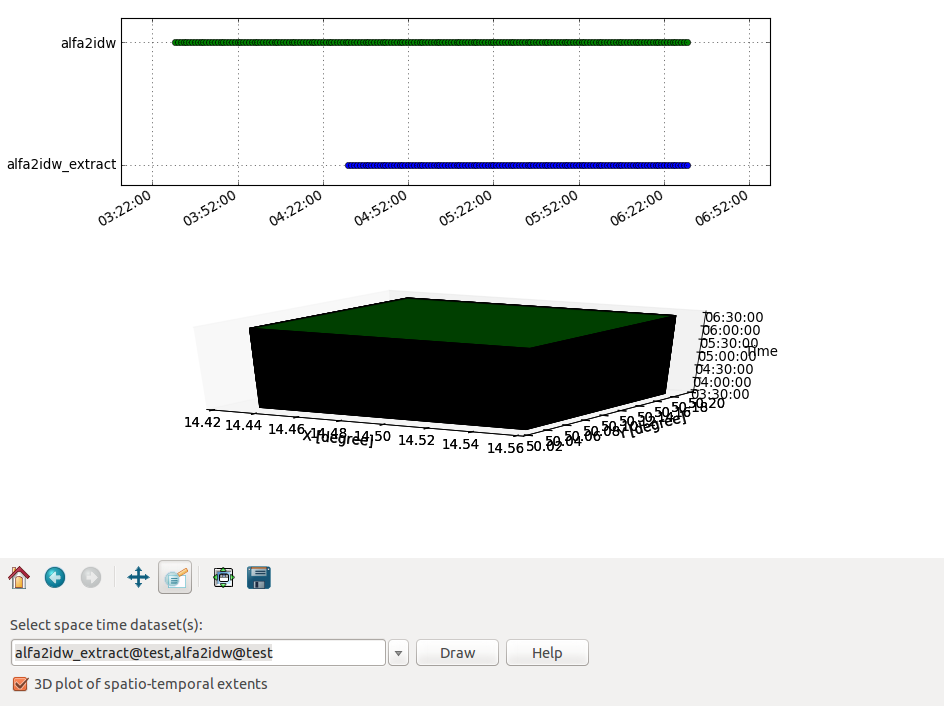
\includegraphics[width=0.6\textwidth]{./img/temporal/timeline.png}
    \caption[Timeline]{\centering  Modul g.gui.timeline pro grafický náhled časových datasetů}
 \end{figure}  


\subsubsection*{Základní analýzy}
\label{subsubsec:casoprostoranal} 


\paragraph{Agregační funkce} slučují buňky o stejných rastrových souřadicích do jednoho rastru, na základě zvolené matematické funkce(průměr, suma, max, min atd.). Rastry jsou slučovány podle zvoleného časového kroku.

Modul, který představuje agregační funkcionalitu se jmenuje t.rast.aggregate\footnote{\url{http://grass.osgeo.org/grass70/manuals/t.rast.aggregate.html}}.  Vytvořený dataset \emph{temporalLetnany}

Agregační funkcí byly vytvořeny rastry reprezentující sumy srážkových intenzit po 15 minutách.
\begin{figure}[h!]
\begin{footnotesize}
\lstset{extendedchars=false,
escapeinside=''}
\begin{lstlisting}[style=mybash]
t.rast.aggregate input=temporalLetnany output=temporal_aggreg \
       basename=sum15minute granularity=15 minutes method=sum
\end{lstlisting}
\end{footnotesize} 
\end{figure}
Jinou agregační funkcí je \textit{t.rast.aggregate.ds}, která má na vstupu dva datasety \emph{a} a \emph{b}. Funkci této agregační funkce je agregace  datasetu \emph{a} podle druhého\emph{ b}, tedy vytvoření časové topologie \emph{a} podle předlohy \emph{b}.



Možností je \textit{r.rast.series}, který využívá k agregaci jiných algoritmů a je určen pro analýzu celého datasetu bez zvolené granularity.
Příkladem je vytvoření rastru s maximálními intenzitami srážek v celém časovém intervalu datasetu. Byly vytvořeny maximální intenzity datasetu s plošnými interpolacemi z 1 bodu nahrazujícího MV spoj s využitím metody RST a IDW


\begin{figure}[h!]
\begin{footnotesize}
\lstset{extendedchars=false,
escapeinside=''}
\begin{lstlisting}[style=mybash]
t.rast.series input=idwt method=maximum output=idwt_seriesmax           
t.rast.series input=rstt method=maximum output=rstt_seriesmax    
\end{lstlisting}
\end{footnotesize} 
\end{figure}

\begin{figure}[h!]
    \centering
    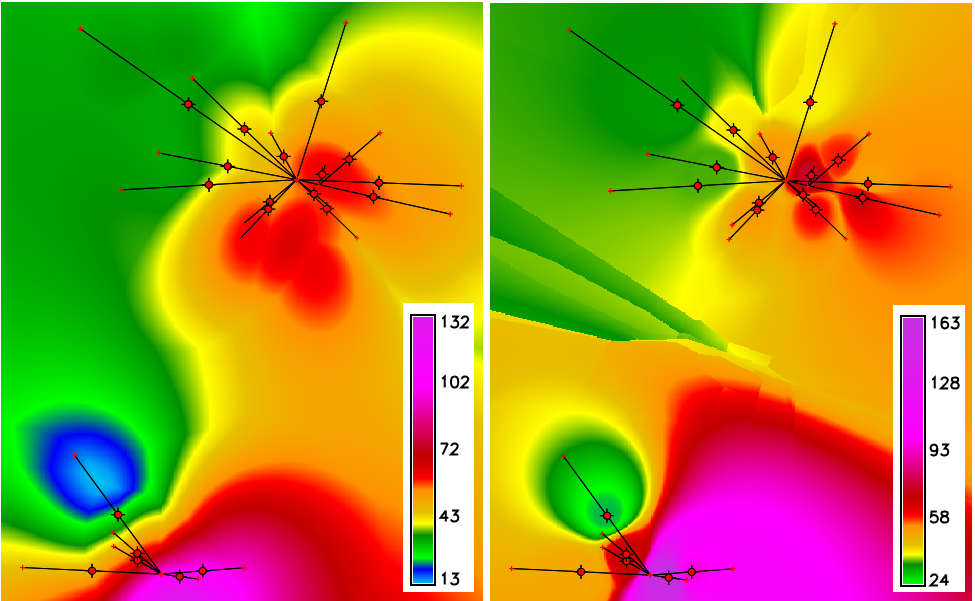
\includegraphics[width=0.6\textwidth]{./img/analys/maxserie.png}
    \caption[Serie max]{Srážková maxima z celého časového datasetu; 1. metoda RST 2. metoda IDW  \centering  }
        \label{fig:baseline}
 \end{figure}



\paragraph*{Mapová algebra}
Mapová algebra se v rámci TGRASS dělí na dva typy
\begin{description}
\item [t.rast.mapcalc] plně podporuje funkcionalitu mapové algebry \textit{r.mapcalc}. Z časoprostorového modelu podporuje například start\_time, end\_time, které jsou nejčastěji využívané.
\item [t.rast.mapcalc2] umožňuje využívat časoprostorové algebry, která je vůbec první svého druhu.
\end{description}

Použití \textit{t.rast.mapcalc} je analogické pro klasickou mapovou algebru v GRASS s rozdílem, že do vypočtu nevstupují jednotlivé rastry ale časové datasety.



\paragraph{Statistické informace } jednotlivých rastrů v časovém datasetu jde vypsat pomocí modulu \textit{t.rast.univar}. Modul  vypíše po jednotlivých řádcích pro dané rastry jejich základní statistické charakteristiky. Pro výpis ve formátu s hlavičkou charakterizující dané hodnoty je možné využít přepínač \texttt{-h}.

\begin{figure}[h!]
\begin{footnotesize}
\lstset{extendedchars=false,
escapeinside=''}
\begin{lstlisting}[style=mybash]
id|start|end|mean|min|max|mean_of_abs|stddev|variance|coeff_var|\
sum|null_cells|cells|first_quartile|median|third_quartile|percentil

alfa1.lview2013_09_09_00_01_rst@test4|2013-09-09 00:01:00\
|None|0|0|0|0|0|0|-nan|0|0|242109|0|0|0|0
    
\end{lstlisting}
\end{footnotesize} 
\end{figure}


\paragraph{Observace}
Vytvoření vektorové vrstvy, která zaznamenává do atributových tabulek údaje z o hodnotách z daného místa napříč časovým datasetem umožňuje modul \textit{t.vect.observe.strds}.

Při volbě observačních bodů v místech dostupných referenčních srážkoměrů, umožní porovnání interpolovaných bodů s referencí.Vektorovou vrstvu je možné zvolit buď z tabulky srážkoměrů, nebo přidat jednotlivé body s využitím modulu \textit{v.in.ascii}
\begin{figure}[h!]
\begin{footnotesize}
\lstset{extendedchars=false,
escapeinside=''}
\begin{lstlisting}[style=mybash]
#P'ř'id'á'n'í' vektorov'é' bodov'é' vrstvy
v.in.ascii input=
  1|50.152761|14.506575
  2|50.141651|14.519106
  3|50.133124|14.501339
  
  output=srazkomery 
  columns=id text,y double precision,x double precision 
  x=3 y=2
\end{lstlisting}
\end{footnotesize} 
\end{figure}

Dalším krokem je nastavení parametru modulu
\begin{figure}[h!]
\begin{footnotesize}
\lstset{extendedchars=false,
escapeinside=''}
\begin{lstlisting}[style=mybash]
t.vect.observe.strds input=srazkomery strds=idw_gama\
  output=observace vector_output=observace_vec columns=precip
\end{lstlisting}
\end{footnotesize} 
\end{figure}

Ve zvolené výchozí databázi se vytvoří časová okna v časovém kroku granularity datasetu.

\subsubsection*{Analýzy}
Kapitola je demonstrativního charakteru, poukazující na možné směry využití výsledku z modul r.mwprecip, kterých je nespočetně mnoho, k čemž přispívá možnost skriptovacího Python API nebo objektového pyGRASS. 

\paragraph*{Suma z plošných interpolací}
Modulm \emph{r.mwprecip} jsou vygenerována minutová časová okna z jednoho dne. Z oken byly interpolovány plošné srážkové intenzity metodou RST a IDW. Cílem analýzy je vytvořit rastr, který bude charakterizovat sumu srážek z intervalu 3 hodin z obou interpolačních metod a tyto rastry od sebe odečteme a spočteme objem vody z rozdílu.


\begin{figure}[h!]
\begin{footnotesize}
\lstset{extendedchars=false,
escapeinside=''}
\begin{lstlisting}[style=mybash]
#Vytvo'ř'en'í' datasetu
t.create output=rst_gama semantictype=mean title=Letnany
t.create output=idw_gama semantictype=mean title=Letnany

#Registrace map 
t.register input=idw_gama@test file=timewin_l_idw
t.register input=rst_gama@test file=timewin_l_rst

#Kontrola
t.info input=rst_gama@test                                                      
t.info input=idw_gama@test

#Vytvo'ř'en'í'  subdataset'ů'
t.rast.extract input=idw_gama@test where=(start_time>2013-09-09\
   03:30:00) and (start_time<'2013-09-09 06:30:00') \
   output=idw_gama_extract
t.rast.extract input=rst_gama@test where=(start_time>2013-09-09\
   03:30:00) and (start_time<'2013-09-09 06:30:00') \
   output=rst_gama_extract

#Suma za 3 hodiny
t.rast.aggregate input=idw_gama_extract@test output=\
   idw_gama_extract_aggbasename=gama3aggidw granularity=3 \
   hours method=sum
t.rast.aggregate input=rst_gama_extract@test output=\
   rst_gama_extract_agg basename=gama3aggrst granularity=3 \
   hours method=sum

#Pr'ů'm'ě'r ze dvou map
t.rast.mapcalc inputs=idw_gama_extract_agg@test,\
   rst_gama_extract_agg@test expression=(idw_gama_extract_agg@test+\
   rst_gama_extract_agg@test)/2 output=gamaSUM basename=gama_sum
\end{lstlisting}
\end{footnotesize} 
\end{figure}



\begin{figure}[h!]%
    \centering
    \subfloat[RST]{ 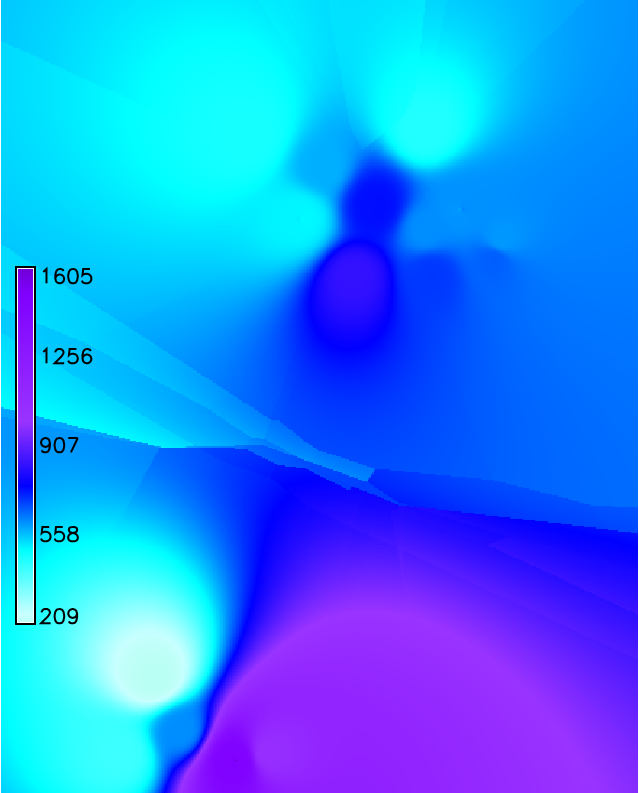
\includegraphics[width=0.27\textwidth]{./img/intanalys/sumrst.png} }%
    \qquad
    \subfloat[IDW]{ 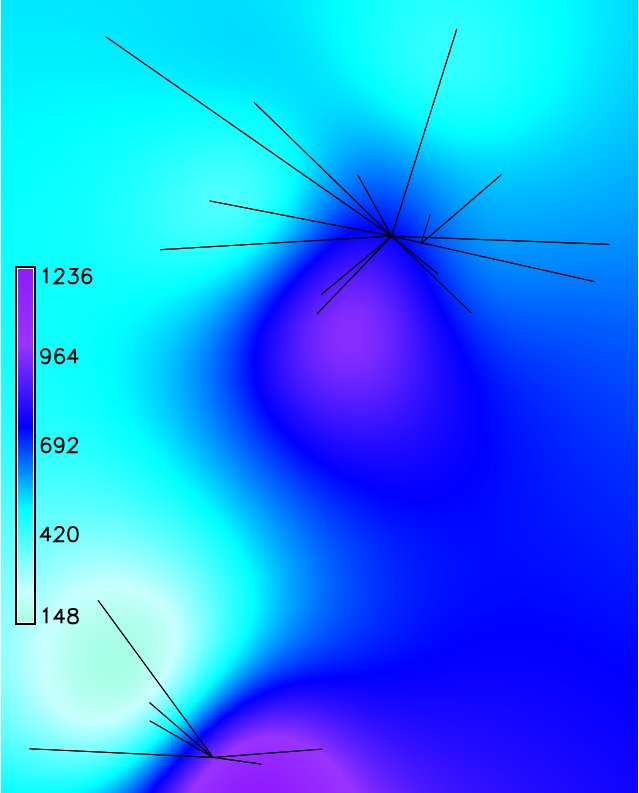
\includegraphics[width=0.27\textwidth]{./img/intanalys/sumidw.png} }%
    \qquad
    \subfloat[Průměr]{ 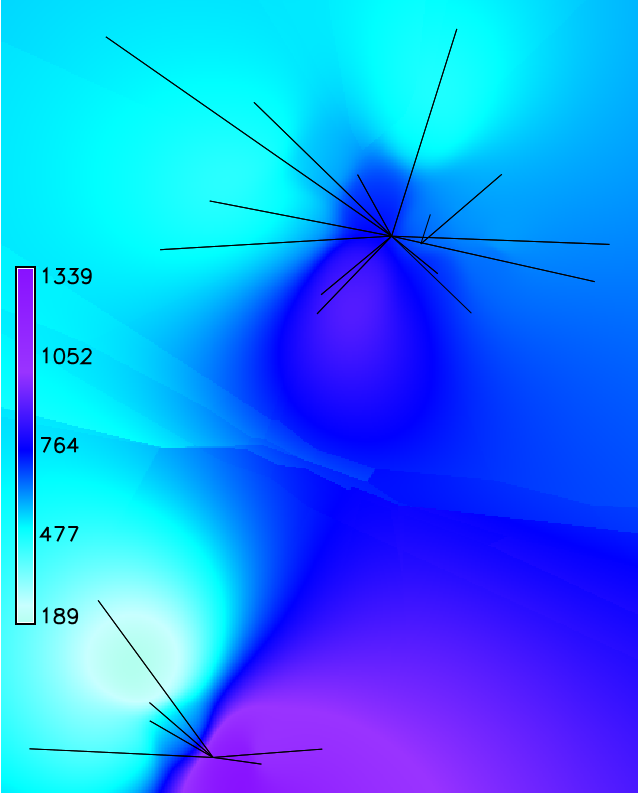
\includegraphics[width=0.27\textwidth]{./img/intanalys/sumavg.png} }%
    \caption[Průměr metod]{ C) rastr vyjadřuje úhrn srážek za 3 hodiny zprůměrovaný z dvou interpolačních metod v [$mm$]\centering}

\end{figure}
Důležité je nezapomenout, v jakých jednotkách rastry byly před vstupem do agregace a v jakých jednotkách jsou poté.
Okna z r.mwprecip  byly v [$mm \cdot h^{-1}$ po jedné minutě, abychom počítaly s reálnými úhrny převedeme na [$mm \cdot min^{-1}$].
Pro porovnání obou interpolačních metod je možné v \textit{r.mapcalc} vytvořit rastr, jehož buňky představují absolutní hodnotou rozdílu dvou interpolačních metod. Modulem \textit{r.univar} spočteme základní statistické charakteristiky včetně sumy všech buněk rozdílného rastru. Ta charakterizuje objemovou odchylku dvou rastrů ze tří hodin v [$mm$] ze zvoleného regionu.


\begin{figure}[h!]
    \centering
    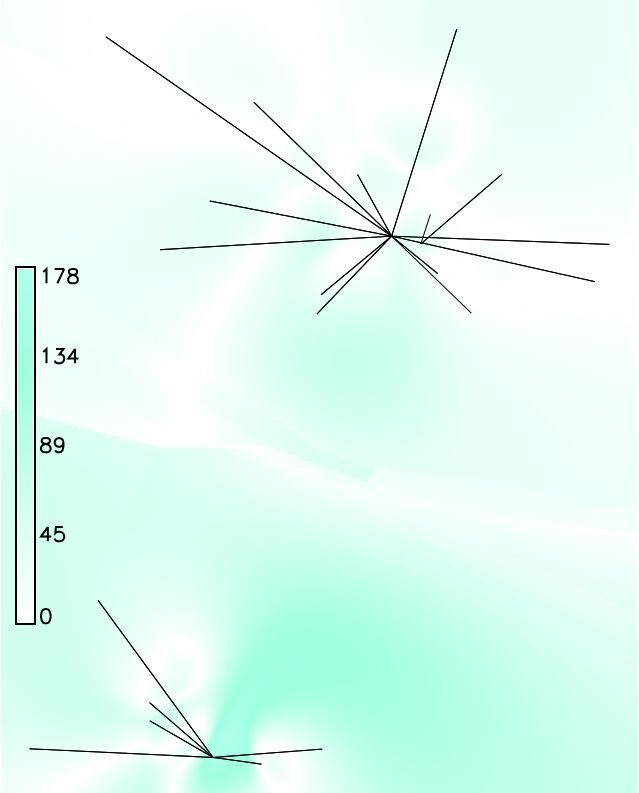
\includegraphics[width=0.27\textwidth]{./img/intanalys/rozdil.png}
    \caption[GUI modul]{Rozdíl dvou rastrů  \centering  }
        \label{fig:baseline}
 \end{figure}
 
Analýza demonstruje agregaci pouze do jednoho časového okna (rastru). V případě, že bychom chtěli vytvořit  agregaci po třech hodinách z intervalu několika dní, k poslednímu kroku bychom využili t.rast.mapcalc namísto standardní r.mapcalc.

\paragraph*{Transformace srážek do povodí}
Vytvoření GIS modulu pro přenesení hrubých dat do formy vypočtených srážek v GIS prostředí bylo prvním a potřebným krokem k dalšímu možnému vývoji jiných GIS modulů. Jedním z možných směrů je automatická klasifikace a transformace srážek do definovaných subpovodí, které by byly vstupem pro srážko-odtokový hydrologický model.

Zjednodušená varianta úlohy demonstruje využití funkcí GRASS a TGRASS pro transformaci srážek do subpovodí. Postup je následující:

\begin{enumerate}
\item r.mwprecip- vytvoření plošných interpolací
\item TGRASS- t.create, t.register a t.rast.aggregate
\item r.in.ogr import \acs{DMT}
\item r.watershed vytvoření subpovodí z DMT
\item r.volume
\end{enumerate}

\begin{enumerate}

\item Prvním krokem je vytvoření plošných interpolací z modulu \textit{r.mwprecip}. 

\begin{figure}[h!]
\begin{footnotesize}
\lstset{extendedchars=false,
escapeinside=''}
\begin{lstlisting}[style=mybash]
r.mwprecip.py -g database=letnany baseltime=/adresar/norain\
       interval=minute lignore=/adresar/ignore pmethod=count\ 
       step=1 
\end{lstlisting}
\end{footnotesize} 
\end{figure}
Vstupem do parametru \texttt{baseltime} jsou dva  časové intervaly období sucha vyplývající z měření srážkoměrů. Sumy srážek jsou vytvořeny po 1 minutě. Do parametru \texttt{lignore} vstupuje soubor s definovanými spoji (linkid), které vykazují vysokou chybovost. Linie spojů byli nahrazeny jedním bodem v pulce, ze kterých se interpoluje explicitně nastavenou interpolací RST. Výpočetní region je nastaven automaticky.


\item Následuje založení časového datasetu, registrace map a agregace po 15 minutách s funkcí sumace \ref{subsubsec:casoprostoranal}

\item Modul \texttt{r.in.gdal} umožňuje importovat rastrová data většiny obecně známých formátů.  Model terénu ze \ac{SRTM}\footnote{\url{http://edcftp.cr.usgs.gov/pub/data/}}, je využit k vytvoření akumulace vody a z té vyplývající jednotlivá povodí v následujícím kroku.

\item Modul \textit{r.watershed } umožňuje vytvoření teoretické vodní sítě, která je odvozena ze sklonu terénu. Jednotlivé vodní sítě představují teoretickou akumulaci vody. Z ní je možné určit subpovodí. Tento krok nám umožňuje demonstrovat úlohu bez dostupných reálných vektorových vrstev o jednotlivých povodích.
\begin{figure}[h!]
\begin{footnotesize}
\lstset{extendedchars=false,
escapeinside=''}
\begin{lstlisting}[style=mybash]
r.watershed  elevation=dem_srtm threshold=5000\
          accumulation=accumulation basin=basin
\end{lstlisting}
\end{footnotesize} 
\end{figure}
Parametr \texttt{treshold} určuje jemnost segmentace jednotlivých povodí. Menší hodnota vede k většímu počtu povodí.

\item Posledním krokem je spočtení objemu srážek, které spadly do daných povodí. K tomu je vhodné využit  modul \textit{r.volume}, pro který jsou vstupními parametry rastr s hodnotami a rastr s klasifikovanými územími. Pro vstup rastru s hodnotami je použit výstup  rastr z \textit{t.rast.aggregate}. Z názvu \textit{max15minute\_148} není poznat o jaký časový interval se jedná, pro získání této informace je určen modul \textit{t.rast.list}, kde je možné konfigurovat parametry pro vypsání do výstupní řádky. Při spuštění bez volitelných parametrů vypadá výpis následovně.
\begin{figure}[h!]
\begin{footnotesize}
\lstset{extendedchars=false,
escapeinside=''}
\begin{lstlisting}[style=mybash]
sum15minute_103	test3  2013-09-10 01:44:00 2013-09-10 01:59:00
\end{lstlisting}
\end{footnotesize} 
\end{figure}

Odtud lze vybrat mapu z požadovaného intervalu která je vstupem(\texttt{input}) pro \textit{r.volume}. 

\begin{figure}[h!]
\begin{footnotesize}
\lstset{extendedchars=false,
escapeinside=''}
\begin{lstlisting}[style=mybash]
r.volume input=sum15minute_103 clump=basin@test3 \
        centroids=volume output=/adresar/r.volumeinfo
\end{lstlisting}
\end{footnotesize} 
\end{figure}

Výsledkem je vektorová bodová mapa, kde ke každému bodu je připojena tabulka s hodnotami výsledků (sum, avg). Parametr \texttt{output} umožňuje uložení tabulky ve formě textového souboru se statistikami celé plochy výpočetního regionu. Výsledné hodnoty pro jednotlivá povodí nejsou v jednotkách  [$mm \cdot h^{-1}$]. Pro převod na objem vody v [$mm \cdot h^{-1}$] je nutné výsledný objem vydělit počtem minut po kterých proběhla agregace.

\end{enumerate} 

\begin{figure}[h!]
    \centering
    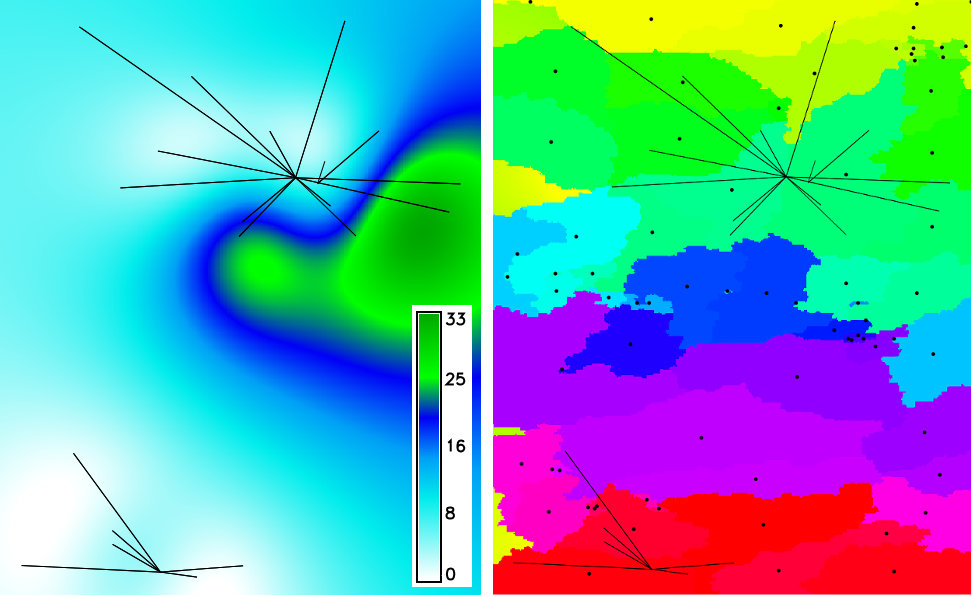
\includegraphics[width=0.6\textwidth]{./img/analys/basin.png}
    \caption[GUI modul]{1. Agregovaný rastr- suma za 15 minut; 2. povodí s bodovou vrstvou představující hodnoty jednotlivých povodí.  \centering  }
        \label{fig:baseline}
 \end{figure}









\setcounter{footnote}{1}
\section{Závěr}
\section{Příloha}
\subsection{Dokumentace}
\subsection{Uživatelská příručka}




%\begin{enumerate*}
   % \item nastavit region na zvolenou rastrovou či vektorovou mapu
    %\item nastavit uložený region (\emph{named region})
   % \item nastavit aktuální výpočetní region
  %  \item zvolit souřadnice středu mapy a měřítko (nastavení regionu
 %   se automaticky vypočítá)
%\end{enumerate*}





\necislovana{Závěr}

Cílem této práce bylo 


\newpage
\necislovana{Seznam použitých zkratek}
\begin{acronym}[USA-CERL]
 	\acro{ANSI}{American National Standards Institute}
  	\acro{API}{Application Programming Interface}
  	\acro{CSV}{Comma Separated Values}
  	
  	\acro{DML}{Data Manipulate on Language}
  	\acro{DSD}{Drop size distribution}
  	\acro{DPZ}{Dálkový průzkum země}
  	\acro{DDL}{Data Definition Language}
  	\acro{DMT}{Digitalní model terénu}
  	\acro{EPSG}{Geodetic Parameter Set}	
  	
  	\acro{GIS}{Geographic Information System (Geografický informační systém)}
  	\acro{GNU GPL}{Všeobecná veřejná licence GNU (GNU General Public License)} 
	\acro{GRASS}{Geographical Resources Analysis Support System}
	\acro{GUI}{Graphical User Interface (Grafické uživatelské rozhraní)}
		
	
	\acro{HMM}{Hidden Markov Model} 
	\acro{IDW}{Inverse Distace Weighting} 
	\acro{IR}{Infra red (infračervené spektrum)} 
	
	\acro{ITU}{International Telecommunication Union}
	
	\acro{OGC}{Open Geospatial Consortium}
	\acro{OSGeo}{Open Source Geospatial Foundation} 
	\acro{ORDBMS}{Object-Relational Database Management System}
	\acro{RGB}{Red Green Blue}
  	\acro{RSL}{Received Signal Level}
  	\acro{STC}{The Space-Time Coposite Data Model}
  	\acro{SRTM}{Shuttle Radar Topography Mission}
    \acro{SRID}{Spatial Reference System Identifier}
	\acro{wxGUI}{WxPython-based GUI for GRASS}	
	
	\acro{WKT}{Well-known text}
\end{acronym}





\newpage
\renewcommand\baselinestretch{1.2}
\selectfont
\renewcommand{\refname}{Použité zdroje}
\phantomsection
\addcontentsline{toc}{section}{\refname}

\begin{thebibliography}{99}
\label{literatura}




\bibitem{radar_meterology}
RAGHAVAN, S. \textit {Radar meteorology}.
31 Oct 2003. Boston: Kluwer Academic Publishers, 2003, 549 s. ISBN 14-020-1604-2. 

\bibitem{flash_floods}
SENE, Kevin. \textit {Flash floods forecasting and warning}.
2013. Dordrecht: Springer, 2013. ISBN 978-940-0751-644. 

\bibitem{vanguard}
GREEN, McLaughlin a Milton LOMASK. \textit {Vanguard - A history: succes - AND AFTER http://history.nasa.gov/SP-4202/toc2.html}.
[online]. [cit. 2014-04-03]. URL:\textless\url {http://history.nasa.gov/SP-4202/chap12.html}

\bibitem{sejong}
STRANGEWAYS, Ian.  \textit {Precipitation: theory, measurement and distribution}.
New York: Cambridge University Press, 2007, x, 290 p. ISBN 978-052-1851-176. 

\bibitem{wmo}
World Meteorological Organization. \textit{Guide to meteorological instruments and methods of observation CHAPTER 6}. WMO-No. 8. Geneva, Switzerland: World Meteorological Organization, 2008. ISBN 978-926-3100-085. 

\bibitem{wren}
ASIT K. BISWAS {Notes and Records of the Royal Society of London: The Automatic Rain-Gauge of Sir Christopher Wren} UK: The Royal Society, 1967. ISSN 00359149. 

\bibitem{sevruk}
SEVRUK, B.\textit{Niederschlag als Wasserkreislauf-element. Theorie und Praxis der Niederschlagsmessung.} 
Zurich-Nitra: Eigenverlag ETH Zurich,  2004, 200 s, ISBN 80–969343–7–6.

\bibitem{chmu_navod}
Česká republika, \textit{Návod pro pozorovatele meteorologických stanic.}
In: Metodický předpis č. 13. Ostrava, 2013. URL:\textless\url {http://old.chmi.cz/OS/pdf/metodicky_navod/MP.pdf}


\bibitem{doppler}
DOVIAK, R. J.; D. S. Zrnic. \textit{Doppler Radar and Weather Observations (2nd ed.)}
(1993), San Diego CA: Academic Press, ISBN 0-12-221420-X.

\bibitem{kohout}
KOHOUT, Jan. \textit{Zpracování a prezentace srážkových dat měřících stanic meteorologického radaru pro ČHMÚ. Informační technologie pro praxi.}
Ostrava: TANGER, 2003. s. 101-103. ISBN 80-85988-90-9.

\bibitem{radar_chmu}
KRÁČMAR, Jan. Český hydrometeorologický ústav. \textit{Meteorologické radiolokátory.} ČHMÚ.
[online]. 1997-2011 [cit. 2014-04-06]. URL:\textless\url {http://portal.chmi.cz/files/portal/docs/meteo/rad/info_radar/index.html}

\bibitem{itu}
RECOMMENDATION ITU-R P.838-3. \textit{Specific attenuation model for rain for use in prediction methods}. 
ITU-R, (1992-1999-2003-2005). URL:\textless\url {https://www.itu.int/dms_pubrec/itu-r/rec/p/R-REC-P.838-3-200503-I!!PDF-E.pdf}

\bibitem{dsd}
CARLTON,W. Ulrich.\textit {Natural Variations in the Analytical Form of the Raindrop Size Distribution}. 
Department of Physics and Astronomy, Clemson University: Journal of Climate and Applied Meteorology, 1983, roč. 1983, č. 22. URL:\textless\url {http://radarmet.atmos.colostate.edu/AT741/papers/Ulbrich_DSD.pdf}

\bibitem{mv1}
ZINEVICH, A., H. MESSER a P. ALPERT. \textit {Prediction of rainfall intensity measurement errors using commercial microwave communication links}. Atmospheric Measurement Techniques [online]. 2010, vol. 3, issue 5, s. 1385-1402 [cit. 2014-04-13]. DOI: 10.5194/amt-3-1385-2010. URL:\textless\url { http://www.atmos-meas-tech.net/3/1385/2010/}

\bibitem{mv2}
MESSER, H. \textit {Environmental Monitoring by Wireless Communication Networks.}, Science [online]. 2006-05-05, vol. 312, issue 5774, s. 713-713 [cit. 2014-04-14]. DOI: 10.1126/science.1120034. URL:\textless\url {http://www.sciencemag.org/cgi/doi/10.1126/science.1120034}

\bibitem{wetat}
M, Schleiss, Rieckermann J. a Berne A.  \textit{Quantification and Modeling of Wet-Antenna Attenuation for Commercial Microwave Links}[online]. 06 únor 2013. Geoscience and Remote Sensing Letters, IEEE, 2013[cit. 2014-04-13]. Volume:10. 

\bibitem{countryw}
OVEREEM, Aart, Hidde LEIJNSE a Remko UIJLENHOET.  \textit{Country-wide rainfall maps from cellular communication networks} [online]. 2012 [cit. 2014-04-13]. 110: 8. DOI: 10.1073/pnas.121796111. URL:\textless\url {http://www.pnas.org/content/110/8/2741.full}

\bibitem{radiolinks}
LEIJNSE, H., R. UIJLENHOET a J. N. M. STRICKER. \textit{Rainfall measurement using radio links from cellular communication networks.} Water Resources Research [online]. 2007, vol. 43, issue 3, n/a-n/a [cit. 2014-04-13]. DOI: 10.1029/2006WR005631. URL:\textless\url {http://doi.wiley.com/10.1029/2006WR005631}

\bibitem{comparsinmv}
Asaf Rayitsfeld, Rana Samuels, Artem Zinevich, Uri Hadar, Pinhas Alpert, \textit{Comparison of two methodologies for long term rainfall monitoring using a commercial microwave communication system}. Atmospheric Research, Volumes 104–105, February 2012, Pages 119-127, ISSN 0169-8095, http://dx.doi.org/10.1016/j.atmosres.2011.08.011.
URL:\textless\url {http://www.sciencedirect.com/science/article/pii/S0169809511002626}

\bibitem{grasshist}
Historical Notes. \textit{GRASS GIS} [online]. 1998-2014 [cit. 2014-04-17]. URL:\textless\url {http://grass.osgeo.org/home/history/}

\bibitem{geospatialanal}
SMITH, Michael J, Michael F GOODCHILD a Paul LONGLEY. \textit{Geospatial analysis: a comprehensive guide to principles, techniques and software tools} [online]. 4th ed. Winchelsea, UK: The Winchelsea Press, c2013, s. 130-135 [cit. 2014-04-18]. ISBN 9781906221980.

\bibitem{gistemporal}
LONGLEY, Paul.\textit{Geographical information systems: principles, techniques, management, and applications}[online]. 2nd ed., abridged. Hoboken, N.J.: John Wiley, c2005., ch 8, [cit. 2014-04-18]. ISBN 0471735450.

\bibitem{lagran}
G. Langran and N.R. Chrisman. \textit{A framework for temporal geographic infor-
mation}. In: Cartographica: The International Journal for Geographic Infor-
mation and Geovisualization 25.3 (1988), pp. 1–14.

\bibitem{hunter}
J. HUNTER, Gary a Ian P. WILLIAMSON. \textit{Journal of Geographic Information System} The Development of a Historical Digital Cadastral Database. 1990, no.2, s. 167-179. URL:\textless\url {http://csdila.unimelb.edu.au/publication/journals/ipw_90_historicalDCDB.pdf}


\bibitem{pelekis}
PELEKIS, Nikos, Babis THEODOULIDIS, Ioannis KOPANAKIS a Yannis THEODORIDIS. Literature Review of Spatio-Temporal Database Models. \textit{The Knowledge Engineering Review}. 2004, September 2004, č. 19, s. 235-274. 

\bibitem{sql1999}
ISO/IEC 9075-2:1999. \textit{Information technology: Database languages SQL}. Part 2: Foundation. SQL/Foundation, 2011. 

\bibitem{postgre}
CHEN, Hao, Heechul HEECHUL a Jin XIAO. \textit{Concept Architecture of PostgreSQL}. 2009. URL:\textit{\url{http://www.inf.fu-berlin.de/lehre/WS09/DBS-Tech/Material/ConceptArchPostres.pdf}}

\bibitem{bares}
BARĚŠ, Pavel. \textit{Implementace materializovaných pohled; v PostgreSQL}. Praha, 2010. Bakalářská práce. ČVUT FIT. Vedoucí práce Ing. Zdeněk Kotala.

\bibitem{sqlmm}
STOLZE, Knut. \textit{SQL/MM Spatial: The Standard to Manage Spatial Data in Relational Database Systems. 2003.}\textless\url {http://doesen0.informatik.uni-leipzig.de/proceedings/paper/68.pdf}



\bibitem{postgis}
CHRISTL, Arnulf.\textit{Introduction to Spatial Data Management with Postgis }
[online]. [cit. 2014-04-20]. URL:\textless\url { http://www.mapbender.org/presentations/Spatial_Data_Management_Arnulf_Christl/Spatial_Data_Management_Arnulf_Christl.pdf}


\bibitem{spatialinter}
Mitas, L., Mitasova, H.,\textit{Geographical Information Systems}
2002; Burrough and McDonnell; Bonham-Carter, 1996, URL: \textless\url {http://csiss.org/learning_resources/content/good_sa/#Interpolation}


\bibitem{spygrass}
GRASS Development Team.\textit{ GRASS 7 Programmer’s Manual}
[online]. c2000-2011, generated on Sat Apr 16 2011 [cit. 2011-03-19]. URL:\textless\url {http://grass.osgeo.org/programming7  }

\bibitem{RST}
HOFIERKA, Jaroslav, Helena  MITASOVA, Lubos MITAS a Juraj PARAJKA.\textit{Multivariate Interpolation of Precipitation Using Regularized Spline with Tension}. Blackwell Publishers Ltd, 108 Cowley Road, Oxford 2002. 

\bibitem{bicubic}
KEYS, R. \textit{ IEEE Transactions on Acoustics, Speech, and Signal Processing}
Cubic convolution interpolation for digital image processing. [online]. 1981, vol. 29, issue 6, s. 1153-1160 [cit. 2014-04-29]. DOI: 10.1109/TASSP.1981.1163711.URL:\textless\url {http://ieeexplore.ieee.org/lpdocs/epic03/wrapper.htm?arnumber=1163711"}




\textless\url {  }

\bibitem{ }
\textit{ }
\textless\url {  }

\bibitem{ }
\textit{ }
\textless\url {  }

\bibitem{ }
\textit{ }
\textless\url {  }

\bibitem{ }
\textit{ }
\textless\url {  }

\bibitem{ }
\textit{ }
\textless\url {  }

\bibitem{ }
\textit{ }
\textless\url {  }

\bibitem{ }
\textit{ }
\textless\url {  }

\bibitem{ }
\textit{ }
\textless\url {  }


\bibitem{ }
\textit{ }
\textless\url {  }





\end{thebibliography}
\end{document}



